%% 
%% Copyright 2007-2020 Elsevier Ltd
%% 
%% This file is part of the 'Elsarticle Bundle'.
%% ---------------------------------------------
%% 
%% It may be distributed under the conditions of the LaTeX Project Public
%% License, either version 1.2 of this license or (at your option) any
%% later version.  The latest version of this license is in
%%    http://www.latex-project.org/lppl.txt
%% and version 1.2 or later is part of all distributions of LaTeX
%% version 1999/12/01 or later.
%% 
%% The list of all files belonging to the 'Elsarticle Bundle' is
%% given in the file `manifest.txt'.
%% 

%% Template article for Elsevier's document class `elsarticle'
%% with numbered style bibliographic references
%% SP 2008/03/01
%%
%% 
%%
%% $Id: elsarticle-template-num.tex 190 2020-11-23 11:12:32Z rishi $
%%
%%
\documentclass[a4paper,12pt]{elsarticle}

%% Use the option review to obtain double line spacing
%% \documentclass[authoryear,preprint,review,12pt]{elsarticle}

%% Use the options 1p,twocolumn; 3p; 3p,twocolumn; 5p; or 5p,twocolumn
%% for a journal layout:
%% \documentclass[final,1p,times]{elsarticle}
%% \documentclass[final,1p,times,twocolumn]{elsarticle}
%% \documentclass[final,3p,times]{elsarticle}
%% \documentclass[final,3p,times,twocolumn]{elsarticle}
%% \documentclass[final,5p,times]{elsarticle}
%% \documentclass[final,5p,times,twocolumn]{elsarticle}

%% For including figures, graphicx.sty has been loaded in
%% elsarticle.cls. If you prefer to use the old commands
%% please give \usepackage{epsfig}

%% The amssymb package provides various useful mathematical symbols
\usepackage{amssymb}
\usepackage{appendix}
\usepackage{comment}
\usepackage{tikz}
\usepackage{tabularx}
\usepackage[hscale=0.8,vscale=0.9]{geometry}
\renewcommand{\deg}{\si{\degree}\xspace} % Use \deg easily, everywhere
\DeclareRobustCommand{\legendsquare}[1]{%
  \tikz[baseline=(a.south)]{\node[#1, inner sep=.8ex, outer sep=0] (a) {};}%
  }
\usepackage{colortbl}
\usepackage{graphics}
\usetikzlibrary{shapes.geometric, arrows, fit}
\usetikzlibrary{arrows.meta}
\usetikzlibrary{automata,positioning}
\usetikzlibrary{shapes.multipart}
\usetikzlibrary{shapes.arrows,calc,positioning}
\definecolor{vent}{RGB}{255, 176, 0}
\definecolor{therm}{RGB}{220, 38, 127}
\definecolor{resp}{RGB}{100, 143, 255}
\definecolor{dyn}{RGB}{254, 97, 0}
\definecolor{TUgreen}{RGB}{108, 194, 74}
\definecolor{TUgreen_pastel}{RGB}{181, 225, 164}
\definecolor{TUblue}{RGB}{0,166,214}
\definecolor{TUblue_pastel}{RGB}{140,199,215}
\definecolor{TUyellow}{RGB}{255, 184, 28}
\definecolor{TUyellow_pastel}{RGB}{252, 216, 142}
\definecolor{TUred}{RGB}{165, 0, 52}
\definecolor{TUviolet}{RGB}{111, 29, 119}
\definecolor{TUorange}{RGB}{237, 104, 66}
\definecolor{TUteal}{RGB}{0,184,200}
\definecolor{TUmarine}{RGB}{0,118,194}
\definecolor{TUocean}{RGB}{0,155,119}

\usepackage{pgfgantt}
\usepackage{nicematrix}
\usepackage{floatrow}
\floatsetup[table]{capposition=top}
\usepackage{comment}
\usepackage{tikz}
\usetikzlibrary{shapes.geometric, arrows}
\tikzstyle{startstop} = [rectangle, rounded corners, minimum width=5cm, minimum height=1cm,text centered, draw=black]
\tikzstyle{io} = [rectangle, minimum width=3cm, minimum height=1cm, text centered,text width=3cm, draw=black]
\tikzstyle{process} = [rectangle, minimum width=3cm, minimum height=1cm, text centered, text width=3cm, draw=black]
\tikzstyle{decision} = [diamond, minimum width=3cm, minimum height=1cm, text centered,text width=3cm, draw=black]
\tikzstyle{arrow} = [thick,->,>=stealth]
\usetikzlibrary{mindmap}
\usepackage{optidef}
\usepackage{siunitx}
\usepackage{longtable}
\setlength\parskip{\smallskipamount}
\DeclarePairedDelimiterXPP\BigOSI[2]%
  {\mathcal{O}}{(}{)}{}%
  {\SI{#1}{#2}}
\usepackage{scalefnt}
\usepackage{mathtools}
\usetikzlibrary{shapes.geometric, arrows, fit}
\usetikzlibrary{automata,positioning}
\usetikzlibrary{shapes.multipart}
\usetikzlibrary{shapes.arrows,calc,positioning}
%% The amsthm package provides extended theorem environments
%% \usepackage{amsthm}

%% The lineno packages adds line numbers. Start line numbering with
%% \begin{linenumbers}, end it with \end{linenumbers}. Or switch it on
%% for the whole article with \linenumbers.
%% \usepackage{lineno}

\journal{Building and Environment}

\begin{document}

\begin{frontmatter}

%% Title, authors and addresses

%% use the tnoteref command within \title for footnotes;
%% use the tnotetext command for theassociated footnote;
%% use the fnref command within \author or \address for footnotes;
%% use the fntext command for theassociated footnote;
%% use the corref command within \author for corresponding author footnotes;
%% use the cortext command for theassociated footnote;
%% use the ead command for the email address,
%% and the form \ead[url] for the home page:
%% \title{Title\tnoteref{label1}}
%% \tnotetext[label1]{}
%% \author{Name\corref{cor1}\fnref{label2}}
%% \ead{email address}
%% \ead[url]{home page}
%% \fntext[label2]{}
%% \cortext[cor1]{}
%% \affiliation{organization={},
%%             addressline={},
%%             city={},
%%             postcode={},
%%             state={},
%%             country={}}
%% \fntext[label3]{}

\title{Quantifying airborne transmission in ventilated settings:\\ A review}

%% use optional labels to link authors explicitly to addresses:
%% \author[label1,label2]{}
%% \affiliation[label1]{organization={},
%%             addressline={},
%%             city={},
%%             postcode={},
%%             state={},
%%             country={}}
%%
%% \affiliation[label2]{organization={},
%%             addressline={},
%%             city={},
%%             postcode={},
%%             state={},
%%             country={}}

\author[inst1]{Arghyanir Giri}

\affiliation[inst1]{organization={Department of Architectural Engineering and Technology, Delft University of Technology},%Department and Organization
            addressline={Julianalaan 134}, 
            city={Delft},
            postcode={2628BL}, 
            state={Zuid Holland},
            country={The Netherlands}}

\author[inst2]{Clara García-Sánchez}
\author[inst1]{Philomena M. Bluyssen}

\affiliation[inst2]{organization={Department of Urbanism, Delft University of Technology},%Department and Organization
            addressline={Julianalaan 134}, 
            city={Delft},
            postcode={2628BL}, 
            state={Zuid Holland},
            country={The Netherlands}}

\begin{abstract}
%% Text of abstract
As the world emerges from the COVID-19 pandemic, mandatory masking and social distancing are becoming increasingly obsolete. Crowded indoor spaces are becoming more common, leaving us vulnerable to future outbreaks. However, ventilation is one widely suggested mitigation measure that did not lose relevance with the pandemic. The airborne transmission of pathogens in indoor ventilated settings has become a significant concern thanks to its profound impact on public health guidelines, building design, and disease control. This review aims to understand the different ventilation solutions in indoor environments used to minimise airborne transmission. Knowing the airflow distribution in a room full of occupants can help design better ventilation strategies and thus reduce the risk of exposure to pathogens. This review systematically reviewed studies linking indoor airflow patterns with droplet distribution. The physics of airflow and droplets are discussed along with the approaches from previous studies that try mimicking them. It is found that social settings have not received proper attention, and some previous assumptions limit the understanding of indoor airborne transmission.
\end{abstract}

\begin{comment}
%%Graphical abstract
\begin{graphicalabstract}

\includegraphics{grabs}
\end{graphicalabstract}

%%Research highlights
\begin{highlights}
\item Research highlight 1
\item Research highlight 2
\end{highlights}
\end{comment}

\begin{keyword}
%% keywords here, in the form: keyword \sep keyword
Airborne transmission \sep Ventilation \sep Multiphase fluid dynamics \sep Respiratory flows \sep Indoor Turbulence

\begin{comment}
  %% PACS codes here, in the form: \PACS code \sep code
\PACS 0000 \sep 1111
%% MSC codes here, in the form: \MSC code \sep code
%% or \MSC[2008] code \sep code (2000 is the default)
\MSC 0000 \sep 1111  
\end{comment}

\end{keyword}

\end{frontmatter}

%% \linenumbers

%% main text
\section{Introduction}
\label{sec:sample1}

Since the onset of the COVID-19 pandemic, over 600 million people are confirmed to have been infected by the SARS-CoV-2 virus, and over 6 million people have lost their lives as of last December 2023 \cite{world2023therapeutics}. A boom in scientific research focused on containing, limiting, and mitigating the spread of the SARS-CoV-2 virus was observed since the outbreak began in Wuhan in early 2020 \cite{morawska2020can,morawska2020time}. Numerous scientists made a critical suggestion that the concerned virus is airborne-spread \cite{zhang2020identifying,bazant2021guideline,morawska2020airborne}. Fortunately, the outbreak was managed with the help of public health guidelines on mandating masks, contact tracing, and social distancing. However, there was some resistance and debate on its transmission route as it was initially believed to be a droplet-spread disease that limited the transmission routes to coughing, sneezing, and direct inhalation from contaminated surfaces \citep{chagla2021re}. It took some time for health advice to catch up with the scientific findings as WHO took almost 2 years to include `long-range airborne transmission' in their official statements \cite{lewis2022took}. 

One of the steps taken to curb the spread of SARS-CoV-2 was the use of sufficient ventilation as it has proven to be an effective measure to curb the spread of viruses \cite{ren2021numerical}, pathogens \cite{berrouk2010experimental} or contaminants \cite{li2020investigating}. Many studies have suggested that long-range transmission occurred inside poorly ventilated settings in the initial stages of the COVID-19 pandemic \cite{morawska2020can,li2021probable, liu2021simulation}. As most public health guidelines have been eased now and everyone is leading their lives normally, studying the airborne transmission of pathogens at this point is not an analysis of what happened in the past but a preparation for the next pandemic ahead of us. Therefore, the role of indoor ventilation in minimising infection risk cannot be understated in the current scenario.

While researchers unanimously agree that indoor environments require sufficient ventilation, increasing the room's air change per hour (ACH) will not reduce the risk of exposure to pathogen-laden droplets. Some more nuances in ventilating a room still need to be addressed. Although a high ACH helps with the removal of pathogens in a room \cite{guo2022visualization, ho2021modeling}, it does not necessarily reduce the droplet concentration near an occupant \cite{arpino2023cfd}. Additionally, recirculating the same air within the room without proper filtering or treatment is another flaw in current ventilation systems \cite{li2021probable}. There is an urgent need to develop methods to predict and quantify the airborne transmission potential of viruses based on model studies, experiments and outbreak research. The present study is a systematic review of research on expelled respiratory droplets in a ventilated setting and the associated risk of infection. This review aims to understand different ventilation regimes and their effect on airflow and droplets to minimise airborne transmission of pathogens.

Previously, airborne transmission in an indoor environment has been looked at from epidemiological, biological, physical, and computer modelling perspectives \cite{argyropoulos2023airborne}. The studies focused on modelling highlighted common limitations like averaging the effects of turbulence \cite{mirzaie2021covid,dbouk2020respiratory},  neglecting the effects of small-scale eddies, and using tracer gases to understand aerosol dynamics that fail to capture properties like volatility and deposition on surfaces \cite{rayegan2022review, zhao2022airborne}. The importance of ventilation design is illustrated by various reviews like \cite{luongo2016role}, \cite{hobeika2023assessing} \& \cite{thornton2022impact}, which show how good ventilation design mitigates transmission, while \citet{correia2020airborne} suggest how bad ventilation can become a reason for long-range transmission. The medical setting has been a major subject of research in this field. Classroom and office room settings have received some attention among non-medical settings. Unfortunately, the distribution of infectious aerosol droplets in ventilated social settings has been rarely looked at despite their interesting change in behaviour with size.

\section{Methods}

For the review, Web of Science, Scopus, and PubMed were chosen as the databases for searching relevant literature. This review has five broad topics: (a) transmission of the pathogen, (b) ventilation regime, (c) investigation approach, (d) setting, and (e) risk analysis. Keywords are chosen under each broad topic to identify relevant literature in the web databases as shown in Table \ref{tab:keys}. Boolean operators `AND'/`OR' combine the search terms and construct a query. The Boolean operator `OR' combines the keywords of each broad topic to form a search query for the corresponding category. The search query from each category is combined to form a final search query using the `AND' boolean operator. This search query identifies an article through the abstract, title and keywords across all the databases.

The term ``SARS-CoV-2 Transmission" is used under the family of keywords even though this study does not focus only on ``SARS-CoV-2" because of the large number of articles that solely refer to the virus in the past two to three years. Additionally, under the category of `Ventilation', the truncated form ``Ventilat*" is used to identify articles that have used it in a different form, along with terms like ``Air cleaning" and ``Filtration". The latter two are mentioned because of the use of air purifiers instead of conventional ventilation systems in some settings. More truncated forms like ``Model*", ``Simulat*", and ``Experiment*" are used to cover every ending of the root word under the `Investigation' category. Search words like ``Machine learning" and ``Deep learning" are included to look for articles using ML or DL to accelerate CFD.

{\renewcommand{\arraystretch}{1.1}
\begin{table}
    \begin{tabularx}{\textwidth}{|p{2.5cm}|X|p{2.5cm}|X|X|}
    \hline
    \multicolumn{5}{|c|}{\textbf{Broad concepts and Keywords}} \\
    \hline
    \textbf{Transmission} & \textbf{Ventilation} & \textbf{Investigation} & \textbf{Setting} & \textbf{Risk Analysis}\\
    \hline
    Airborne Transmission & Ventilat* & Model* & Indoor setting & Risk Assessment \\
    Aerosol Transmission & Air cleaning & Simulat* & Environment & Infection probability\\
    Indoor Transmission & HVAC & Experiment* & Confined spaces & Exposure \\         
    SARS-CoV-2 Transmission & Air change  & CFD & Office  & Wells-Riley\\        
    Indoor contamination & Filtration & Measurement & Restaurant & Dose-response\\        
    Environmental Transmission & Air distribution & Validation & Classroom & \\  
    Airborne route &  & Estimation & Hospital & \\
     &  & Machine Learning &  & \\
    &  & Deep Learning &  & \\
    \hline
    \end{tabularx}
    \caption{Broad concepts and keywords to construct the search query}
    \label{tab:keys}
\end{table}
}

We found 195 articles from Scopus, 258 from Web of Science, and 159 from PubMed. The duplicate articles are merged to get 385 unique papers from the databases. The initial screening of articles is done by reading titles and abstracts to classify them into different categories. Review papers are segregated from the articles to screen them further for relevant studies. After separating the 38 review articles, the remaining 347 papers are screened to find relevance with pathogen transmission in a ventilated indoor environment. Models based solely on theoretical reasoning, papers dealing with building-scale aerodynamics, papers not mentioning ventilation, purely epidemiological studies, and non-English and non-accessible papers were excluded. After excluding 130 papers that did not meet the first criteria, 218 papers that theoretically, experimentally, or computationally investigated airborne transmission of pathogens are left.

Papers that are numerical simulations that are either paired with or validated against experimental studies are given preference here, thus excluding purely qualitative studies, purely measurement-based studies, Reynolds Averaged Navier-Stokes (RANS) simulations that are not validated or validated against theoretical models, and studies that focus on contaminants that are not droplet-based. An exception is made for some Large Eddy Simulations (LES) or Direct Numerical Simulations (DNS) investigating the spread of pathogens via aerosol droplets but do not model ventilation. Their inclusion is important as they are state-of-the-art when it comes to flow simulations for airborne transmission in ventilated settings. After the initial screening, 50 such research papers were selected for review. 

The segregated 38 review articles are screened further for relevance, of which 13 papers reviewed articles on airborne transmission, approaches of research, and ventilation methods. There are 2046 references in the selected review papers, which are subjected to the same exclusion criteria as the initial screening. After screening review papers, 26 additional research papers are found. The 26 research papers included 5 studies that use DNS and 10 studies that use LES. The final set of articles comprises 76 research papers thoroughly reviewed and analysed in the following sections. The review process is summarised in figure \ref{fig:flowchart}.

\begin{figure}
    \centering
    \tikzstyle{io} = [rectangle, minimum width=3cm, minimum height=1cm, text centered,text width=3cm, draw=black]
\tikzstyle{process} = [rectangle, minimum width=3cm, minimum height=1cm, text centered, text width=5cm, draw=black]
\tikzstyle{decision} = [diamond, minimum width=3cm, minimum height=1cm, text centered,text width=3cm, draw=black]
\tikzstyle{arrow} = [thick,->,>=stealth]
\tikzstyle{myfit1} = [draw,solid,black, inner xsep=25pt, inner ysep=25pt, rounded corners=5pt]
\tikzstyle{myfit3} = [draw,solid,black, inner xsep=10pt, inner ysep=20pt, rounded corners=5pt]
\tikzstyle{myfit4} = [draw,solid,black, inner xsep=10pt, inner ysep=10pt, rounded corners=5pt]
\tikzstyle{myfit2} = [draw,dashed,black, inner xsep=10pt, inner ysep=15pt, rounded corners=5pt]
\tikzstyle{mytitle1} = [draw,solid,black, fill=gray!50, inner sep=5pt]
\tikzstyle{mytitle2} = [draw,solid,black, fill=gray!50, inner sep=3pt]
\resizebox{\textwidth}{!}{\begin{tikzpicture}[thick,scale=0.6,node distance=2cm]
\node (start) [startstop] {\textbf{Airborne transmission in ventilated settings}};
\node (topic1) [io,below of=start,xshift=-7cm,yshift=-0.5cm] {\textbf{Transmission}\\7 keywords combined by OR};
\node (topic2) [io,below of=start,xshift=-3.5cm,yshift=-0.5cm] {\textbf{Ventilation}\\6 keywords combined by OR};
\node (topic3) [io,below of=start,yshift=-0.5cm] {\textbf{Investigation}\\9 keywords combined by OR};
\node (topic4) [io,below of=start,xshift=3.5cm,yshift=-0.5cm] {\textbf{Setting}\\7 keywords combined by OR};
\node (topic5) [io,below of=start,xshift=7cm,yshift=-0.5cm] {\textbf{Risk analysis}\\5 keywords combined by OR};
\node (quer) [io, below of=topic3,yshift=-0.5cm] {Final search query\\combined by AND};
\node (in0) [io, below of=quer,xshift=-3.5cm, yshift=-2cm] {Papers in Scopus\\(n = 195)};
\node (in1) [io, below of=quer,yshift=-2cm] {Papers in WoS\\(n = 258)};
\node (in15) [io,below of=quer,xshift=3.5cm,yshift=-2cm] {Papers in PubMed\\(n = 159)};
\node (in2) [io, below of=in1,yshift=-0.5cm] {Papers after merging duplicates\\(n = 385)};
\node (in3) [io, below of=in2,yshift=-0.5cm] {Non-review articles for screening\\(n = 347)};
\node (in4) [io, below of=in3,yshift=-0.5cm] {Relevant studies\\(n = 218)};
\node (in5) [io, right of=in2,xshift=2.5cm] {Review papers\\(n = 38)};
\node (in6) [io, below of=in4,yshift=-1cm] {Core papers after initial screening\\(n = 50)};
\node (in8) [io, below of=in5,] {Relevant reviews\\(n = 13)};
\node (in10) [io, below of=in8,yshift=-4cm] {Papers from reviews\\(n = 26)};
\node (ex1) [process,left of=in3, xshift = -4cm,yshift=0.8cm] {Excluded studies (n = 130)\\- theoretical models\\- building-scale studies\\- no discussion on ventilation\\- purely epidemiological studies\\- non English papers \\- not accessible};
\node (ex2) [process,left of=in4, xshift = -4cm,yshift = -1.8cm] {Excluded studies (n = 168)\\- unvalidated RANS\\- qualitative studies\\- purely measurement based\\- simulations validated against theoretical models\\- non-droplet contaminant};
\node (ex3) [io, right of=in8,xshift=2cm, yshift=-3.2cm] {Excluded\\references\\(n = 2046)\\-duplicates\\-unvalidated RANS\\-no droplets\\-no ventilation};
\node (cl1) [io, below of=in6,xshift=-4.5cm, yshift=-2cm] {Identifying airflow patterns};
\node (cl2) [io, below of=in6, yshift=-2cm] {Understanding droplet physics};
\node (cl3) [io, below of=in6,xshift=4.5cm, yshift=-2cm] {Reviewing modelling techniques};
\node (end) [startstop, below of=cl2, yshift=-1cm] {Discuss trends, weaknesses and future direction};
 
\draw [arrow] (start) -- node[anchor=west] {} (topic3);
\draw [arrow] (start) -| node[anchor=east] {} (topic1);
\draw [arrow] (start.189) -| node[anchor=east] {} (topic2.north);
\draw [arrow] (start.351) -| node[anchor=east] {} (topic4.north);
\draw [arrow] (start) -| node[anchor=west] {} (topic5);
\draw [arrow] (topic1) |- node[anchor=west] {} ([yshift=0.3cm]quer.west);
\draw [arrow] (topic2) |- node[anchor=east] {} ([yshift=0.3cm]quer.west);
\draw [arrow] (topic3) -- node[anchor=west] {} (quer);
\draw [arrow] (topic4) |- node[anchor=east] {} ([yshift=0.3cm]quer.east);
\draw [arrow] (topic5) |- node[anchor=west] {} ([yshift=0.3cm]quer.east);
\draw [arrow] (quer) -- node[anchor=west] {} (in1);
\draw [arrow] (quer) -| node[anchor=east] {} (in0);
\draw [arrow] (quer) -| node[anchor=west] {} (in15);
\draw [arrow] (in1) -- node[anchor=east] {} (in2);
\draw [arrow] (in0.270) -| node[anchor=east] {} ([xshift=-0.3cm]in2.north);
\draw [arrow] (in15.270) -| node[anchor=east] {} ([xshift=0.3cm]in2.north);
\draw [arrow] (in3) |- node[anchor=east] {} ([yshift=-3.6cm]ex1.east);
\draw [arrow] (in4) |- node[anchor=east] {} ([yshift=0.9cm]ex2.east);
\draw [arrow] (in8) |- node[anchor=east] {} (ex3);
\draw [arrow] (in2) -- node[anchor=west] {} (in3);
\draw [arrow] (in2) -- node[anchor=west] {} (in5);
\draw [arrow] (in3) -- node[anchor=west] {} (in4);
\draw [arrow] (in4) -- node[anchor=west] {} (in6);
\draw [arrow] (in5) -- node[anchor=west] {} (in8);
\draw [arrow] (in8) -- node[anchor=east] {} (in10); 


\node[fit=(topic1)(topic2)(topic3)(topic4)(topic5)(quer),myfit3] (strats) {};
\node[mytitle2] at ([xshift=-7cm]strats.south) {Search strategy};

\node[fit=(in0)(in1)(in15)(in2)(in3)(in4)(in5)(in6)(in8)(in10)(ex1)(ex2)(ex3),myfit3] (screening) {};
\node[mytitle2] at ([xshift=-7cm]screening.south) {Screening};


\node[fit=(cl1)(cl2)(cl3),myfit1] (analysis) {};
\node[mytitle2] at ([xshift=-7cm]analysis.south) {Analysis};
\draw[arrow](analysis) -- node[anchor=east] {} (end);

\node[fit=(in6)(in10),myfit4] (final) {};
\node[mytitle2] at (final.north) {Final set of papers};
\draw[arrow] ([xshift=-3.75cm]final.south) -- (analysis.north);


\end{tikzpicture}}
    \caption{The review process}
    \label{fig:flowchart}
\end{figure}

\section{Outcome of review}

The review summarises studies on common airflow structures found in different ventilated settings, droplet physics in respiratory aerosols for different indoor conditions, and both experimental and simulation studies used to mimic airborne transmission scenarios.

\subsection{Airflow in indoor environments}

Airborne transmission in an indoor environment calls for discussing airflow patterns, which are the bulk carriers of pathogen-laden aerosols. The indoor airflow has multiple components and differs according to the setting, ambient room conditions, and occupancy. Indoor airflow mainly constitutes ventilation flow, flow due to temperature differences, and respiratory flows. Every setting has a unique configuration of occupants, obstructions and ventilation, making their interaction with different respiratory activities interesting. The overlap between different sources of airflow inside various indoor environments is illustrated through Table \ref{tab:mat}, qualitatively highlighting the mixing potential of the flows.

Some common occupant configurations and ventilation regimes were found from the review, from which three of each were selected. The selected occupant configurations and ventilation regimes are represented in a matrix illustrating the variation among the nine scenarios. The scenarios are visualised as simplified schematics roughly adapted from the previous research with different sources of airflow illustrated with different colours. Occupant configuration 1 is where the occupants are facing each other, and occupant configuration 2 is where the occupants are facing the same direction. Occupant configuration 3 is specific to a healthcare setting where one occupant is lying, and another is standing beside them.

The first occupant configuration is observed in hospitals \cite{zhou2021experimental}, offices \cite{li2023numerical}, and restaurants \cite{oksanen2022combining} where the two occupants are sitting facing each other, across a table as shown in the schematics. For this occupant configuration, the respiratory flows (shown in blue) collide head-on and spread axially depending on the offset height and laterally \cite{giri2022colliding, singhal2022virus} while the thermal flows (in red) rise upward with intensity depending on the temperature difference between the surface of the occupant and the ambient temperature \cite{zhang2019distribution}. The second occupant configuration is observed in classrooms \cite{qin2023transmission}, offices \cite{he2011cfd}, and modes of transport \cite{yan2021transmission,ho2021modeling} where the occupants are facing in the same direction. The respiratory flows in this configuration interact directly with the thermal flow \cite{ou2022insufficient}. The third configuration of occupants is unique to hospitals and healthcare buildings where one or more occupants are lying and standing \cite{villafruela2019assessment, lu2020reducing}. The lying occupants are patients, while the standing are healthcare workers or visitors. In this case, the respiratory flow is parallel to the thermal flow, which results in a net upward flow. The surface area of the lying occupant is greater than that of a sitting occupant, resulting in laterally spread thermal plumes \cite{feng2020influence}.

In table \ref{tab:mat}, Ventilation Regime 1 is mixing ventilation, Ventilation Regime 2 is displacement ventilation, and Ventilation Regime 3 is stratum and cross ventilation. With the three different ventilation regimes, different overlaps between the three sources of airflow (differentiated by colour) were observed. From Table \ref{tab:mat}, it is evident that Ventilation regime 1 is the most widely used ventilation regime across all occupant configurations and almost all indoor settings. This is based on the idea that mixing ventilation can dilute the pathogen or pollutant concentration in the room \cite{srivastava2021effective}. Ventilation regimes 2 and 3 are less common in comparison because the indoor airflow is directional, upward and lateral, respectively, making them less versatile in most scenarios but more effective in some.

\begin{table}[ht]
    \caption{Schematics for indoor airflow matrix with three common occupant configurations and three common ventilation regimes. The airflow is differentiated into three types with colours as follows: \legendsquare{fill=resp} Respiratory flow \legendsquare{fill=vent} Ventilation flow \legendsquare{fill=therm} Thermal flow }
    \label{tab:mat}
    \centering
    \begin{tabular}{|m{2.5cm}|m{4cm}|m{4cm}|m{4cm}|}
    \hline
     & \textbf{Ventilation regime 1} & \textbf{Ventilation regime 2} & \textbf{Ventilation regime 3} \\
    \hline
    \textbf{Occupant Configuration 1} & 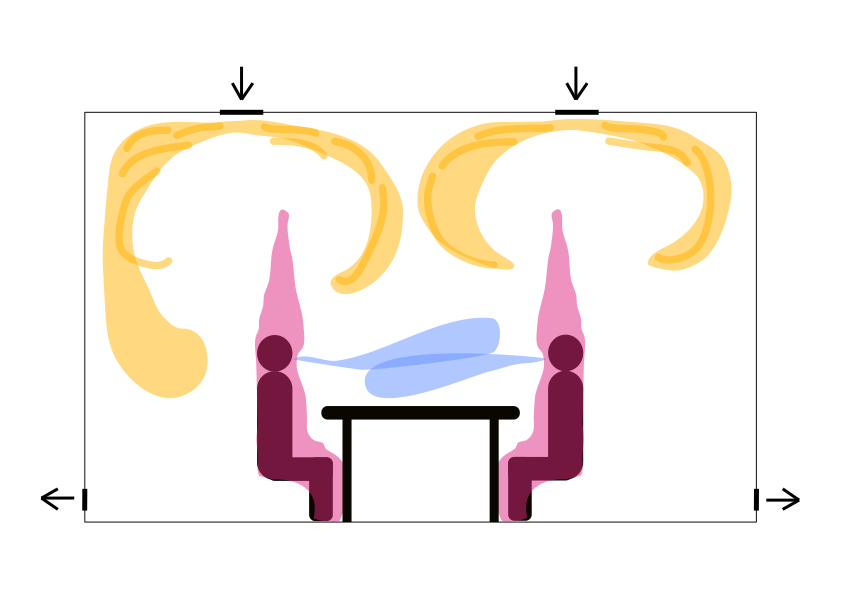
\includegraphics[clip,trim={0 2cm 0 2cm},width=0.25\textwidth]{Airflow/mat1.jpeg}& 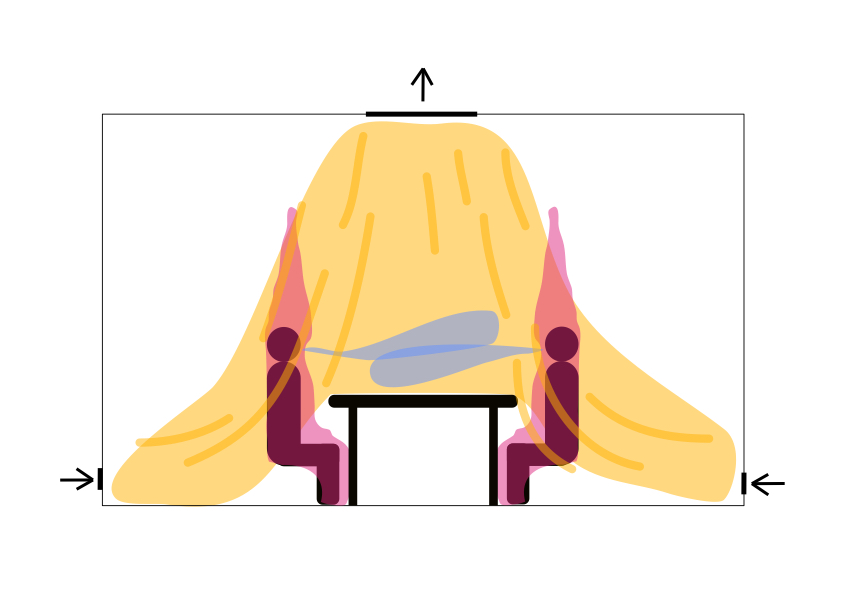
\includegraphics[clip,trim={0 2cm 0 2cm},width=0.25\textwidth]{Airflow/mat4.jpeg}& 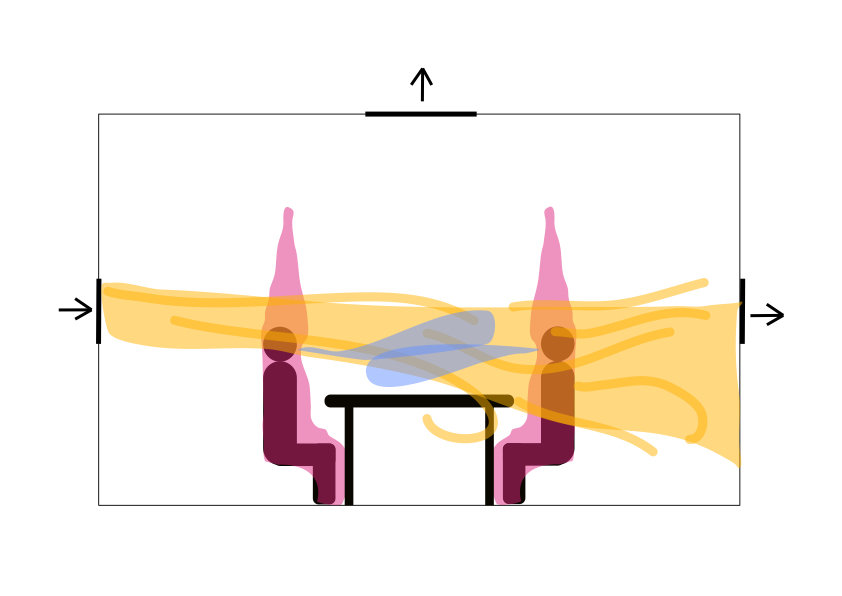
\includegraphics[clip,trim={0 2cm 0 2cm},width=0.25\textwidth]{Airflow/mat7.jpeg} \\
    \hline
    \textbf{References} & \cite{li2020investigating,zhou2021experimental,pan2022boundary,pan2023predicting,li2022airborne} & \cite{deng2021control,zhou2021experimental,wu2023numerical} & \cite{pendar2020numerical,feng2020influence} \\
    \hline
    \textbf{Occupant Configuration 2} &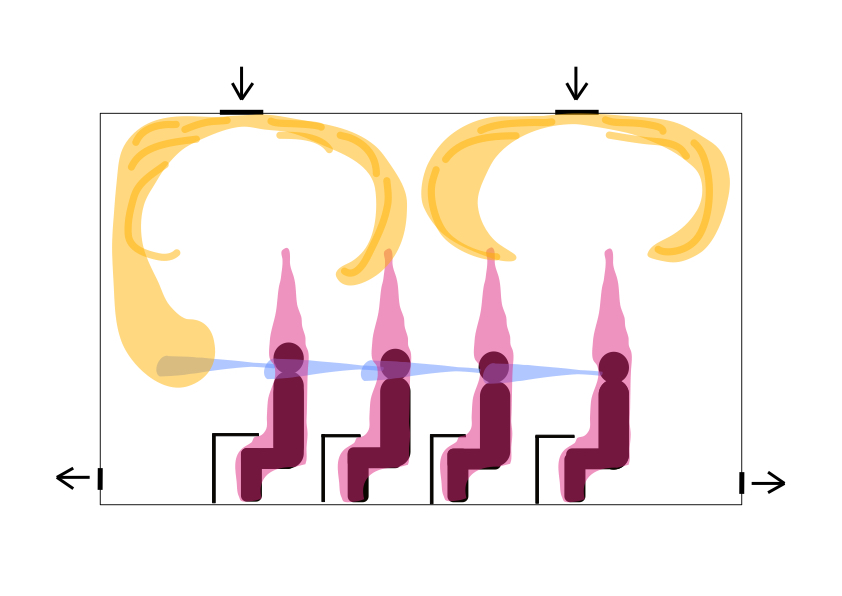
\includegraphics[clip,trim={0 2cm 0 2cm},width=0.25\textwidth]{Airflow/mat2.jpeg}& 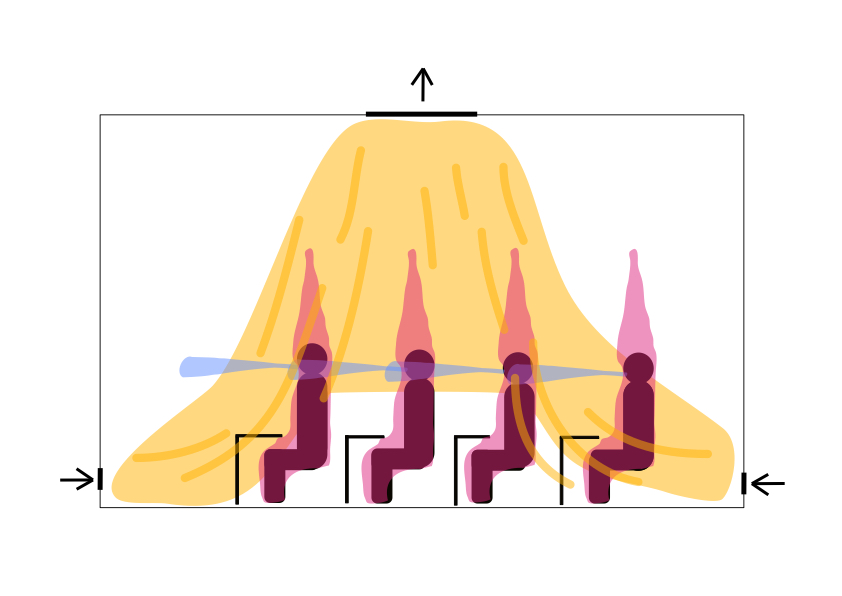
\includegraphics[clip,trim={0 2cm 0 2cm},width=0.25\textwidth]{Airflow/mat5.jpeg}& 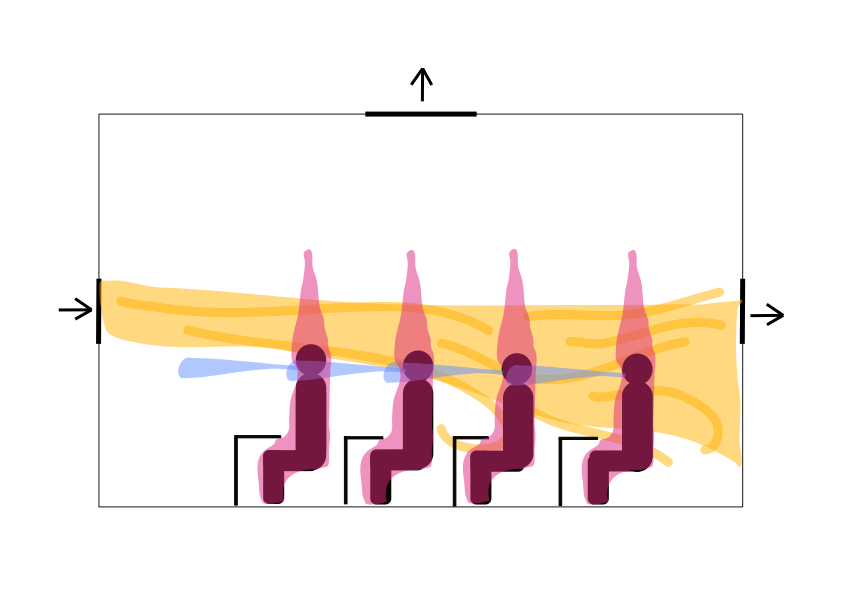
\includegraphics[clip,trim={0 2cm 0 2cm},width=0.25\textwidth]{Airflow/mat8.jpeg} \\
    \hline
    \textbf{References} & \cite{he2011cfd,yan2021transmission,mirzaie2021covid,li2021effects,shao2021risk,qin2023transmission,xu2023cfd} & \cite{he2011cfd,lu2022ventilation,jain2023numerical} & \cite{ho2021modeling,duill2021impact,ren2022practical,lu2022ventilation} \\
    \hline
    \textbf{Occupant Configuration 3} &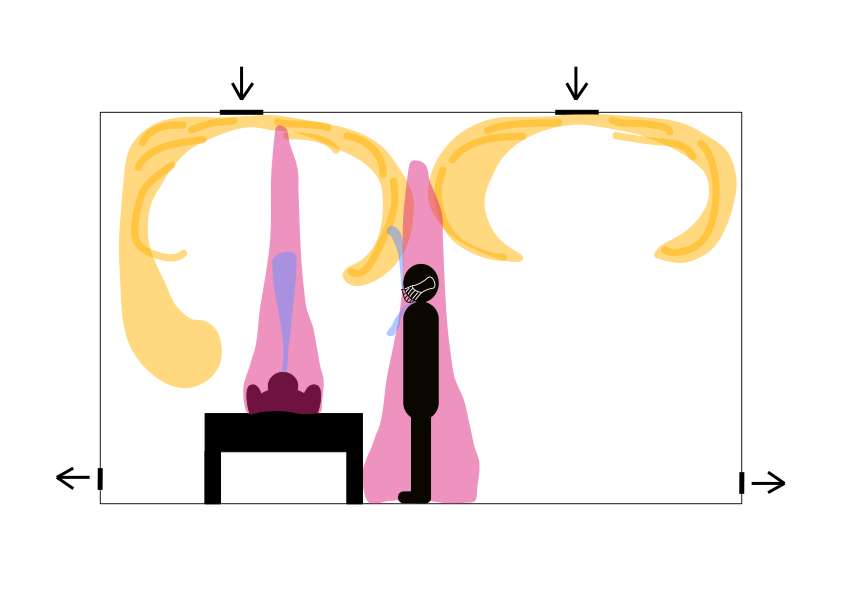
\includegraphics[clip,trim={0 2cm 0 2cm},width=0.25\textwidth]{Airflow/mat3.jpeg}& 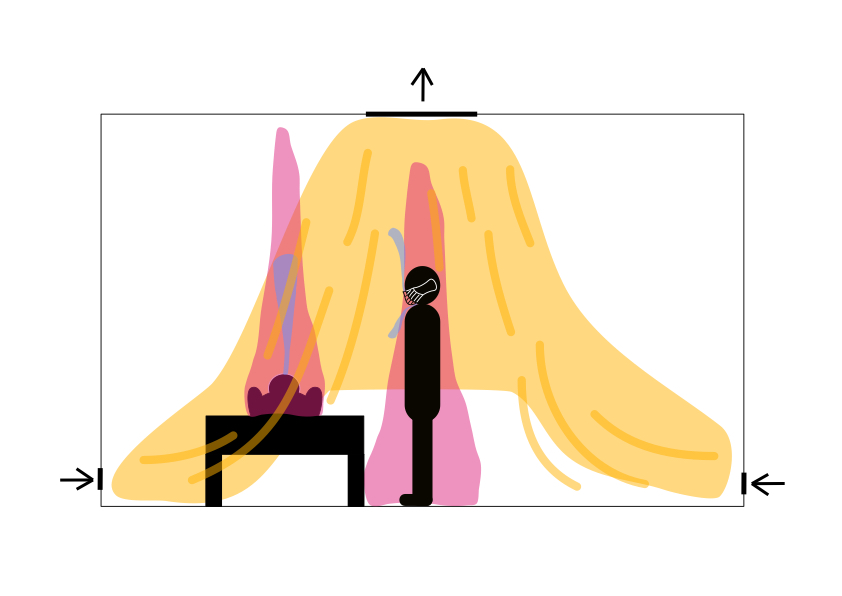
\includegraphics[clip,trim={0 2cm 0 2cm},width=0.25\textwidth]{Airflow/mat6.jpeg}& 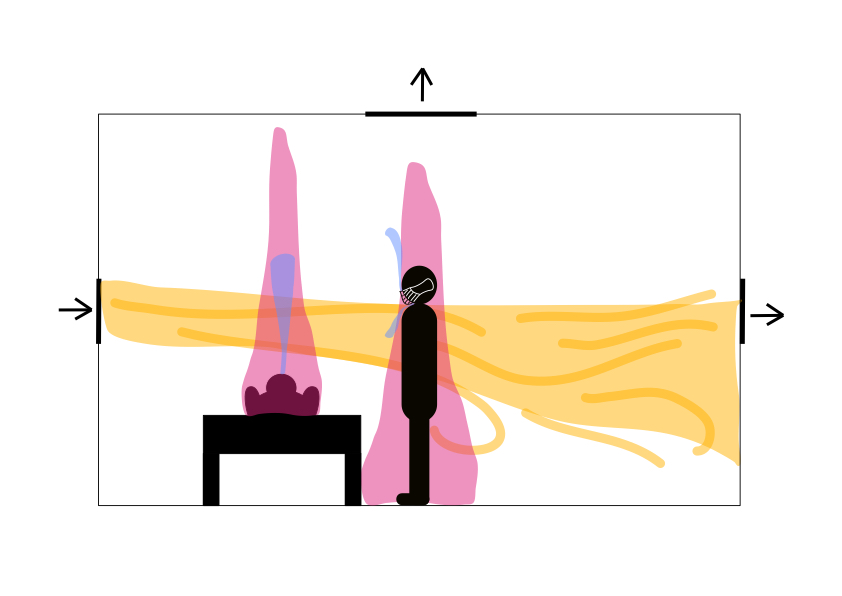
\includegraphics[clip,trim={0 2cm 0 2cm},width=0.25\textwidth]{Airflow/mat9.jpeg} \\
    \hline
    \textbf{References} & \cite{hang2014influence,romano2015numerical,liu2020full,lu2020reducing,zhou2021experimental,guo2022visualization,liu2023estimating} & \cite{zhou2021experimental,villafruela2019assessment,lu2020reducing} & \cite{jiang2009investigating,lu2020reducing} \\
    \hline
    \end{tabular}

\end{table}

\subsection{Droplet dynamics}

Pathogens are ejected via respiratory activity and transmitted from an infected individual to a susceptible one through direct/indirect airborne or fomite transmission \cite{leung2021transmissibility}. In every transmission route, pathogens exist in the form of aerosols, which can evaporate, condense, coalesce, and deposit, making simulating their behaviour complicated \cite{rosti2020fluid,zhou2021dynamical}. The ambient conditions, the type of respiratory activity, and the droplet's size significantly impact their physical behaviour and potential to carry pathogens across space.

Temperature and relative humidity are two primary parameters describing ambient conditions in a room. The room's temperature mainly affects the intensity of thermal currents from the occupants and, consequently, the propagation of respiratory droplets \cite{feng2020study}. Relative humidity mainly affects how long the droplet is suspended in the air, which affects the evolution of the droplet over time. Lower ambient temperatures result in higher buoyancy effects on the exhaled droplets, which lead to their accumulation near the ceiling \cite{zhang2019distribution}. Whereas high relative humidity increases the lifetime of respiratory droplets as small droplets are protected from evaporation by the humid respiratory plume of the occupant \cite{chong2021extended}. The droplet plume schematics in the first two columns of Table \ref{tab:mat2} show the effect on droplet dynamics for different combinations of ambient conditions.

Humans shed droplets during respiratory activities like sneezing, coughing and speech \cite{stadnytskyi2021breathing}. These droplets often differ in velocity, size, and number. The droplets during a cough or sneeze are expelled at high velocities, thus reaching large distances away from the mouth in contrast to droplets expelled during speaking and breathing \cite{pendar2020numerical,zhang2019distribution}. Cough/sneeze droplets are larger in diameter ($ 10-100 \mu m$), while breathing produces relatively smaller droplets $\BigOSI{1}{\mu\meter}$ \cite{shao2021risk}. On the other hand, speech sheds droplets of sizes ranging from $\BigOSI{1}{\mu\meter}$ to $\BigOSI{1}{\milli\meter}$ where the bigger droplets settle down because of gravity while smaller ones follow the airflow \cite{tan2021experimental}. Time scales for sneezing and coughing are quite small $\BigOSI{1}{\second}$. As a result, the number of droplets produced is lower $\BigOSI{1000}{\per\second}$ compared to speech or breathing where the activity can last longer $\BigOSI{1}{\minute}$ thus producing an order of magnitude higher number of droplets $\BigOSI{10000}{\per\second}$ \cite{giri2022colliding}. Furthermore, the production of droplets is higher if the occupant speaks loudly or makes plosive sounds \cite{abkarian2020speech}. The second column in Table \ref{tab:mat2} shows the droplet plume schematics for the four different respiratory activities discussed above with different-sized droplets differentiated with colour.

\begin{table}[h!]
    \centering
    \begin{tabular}{|m{2.5cm}|m{4cm}||m{2.5cm}|m{4cm}|}
    \hline
    \textbf{Ambient conditions} & \textbf{Schematic} & \textbf{Respiratory activity} & \textbf{Schematic} \\
    \hline
    Low temperature \& Low humidity & 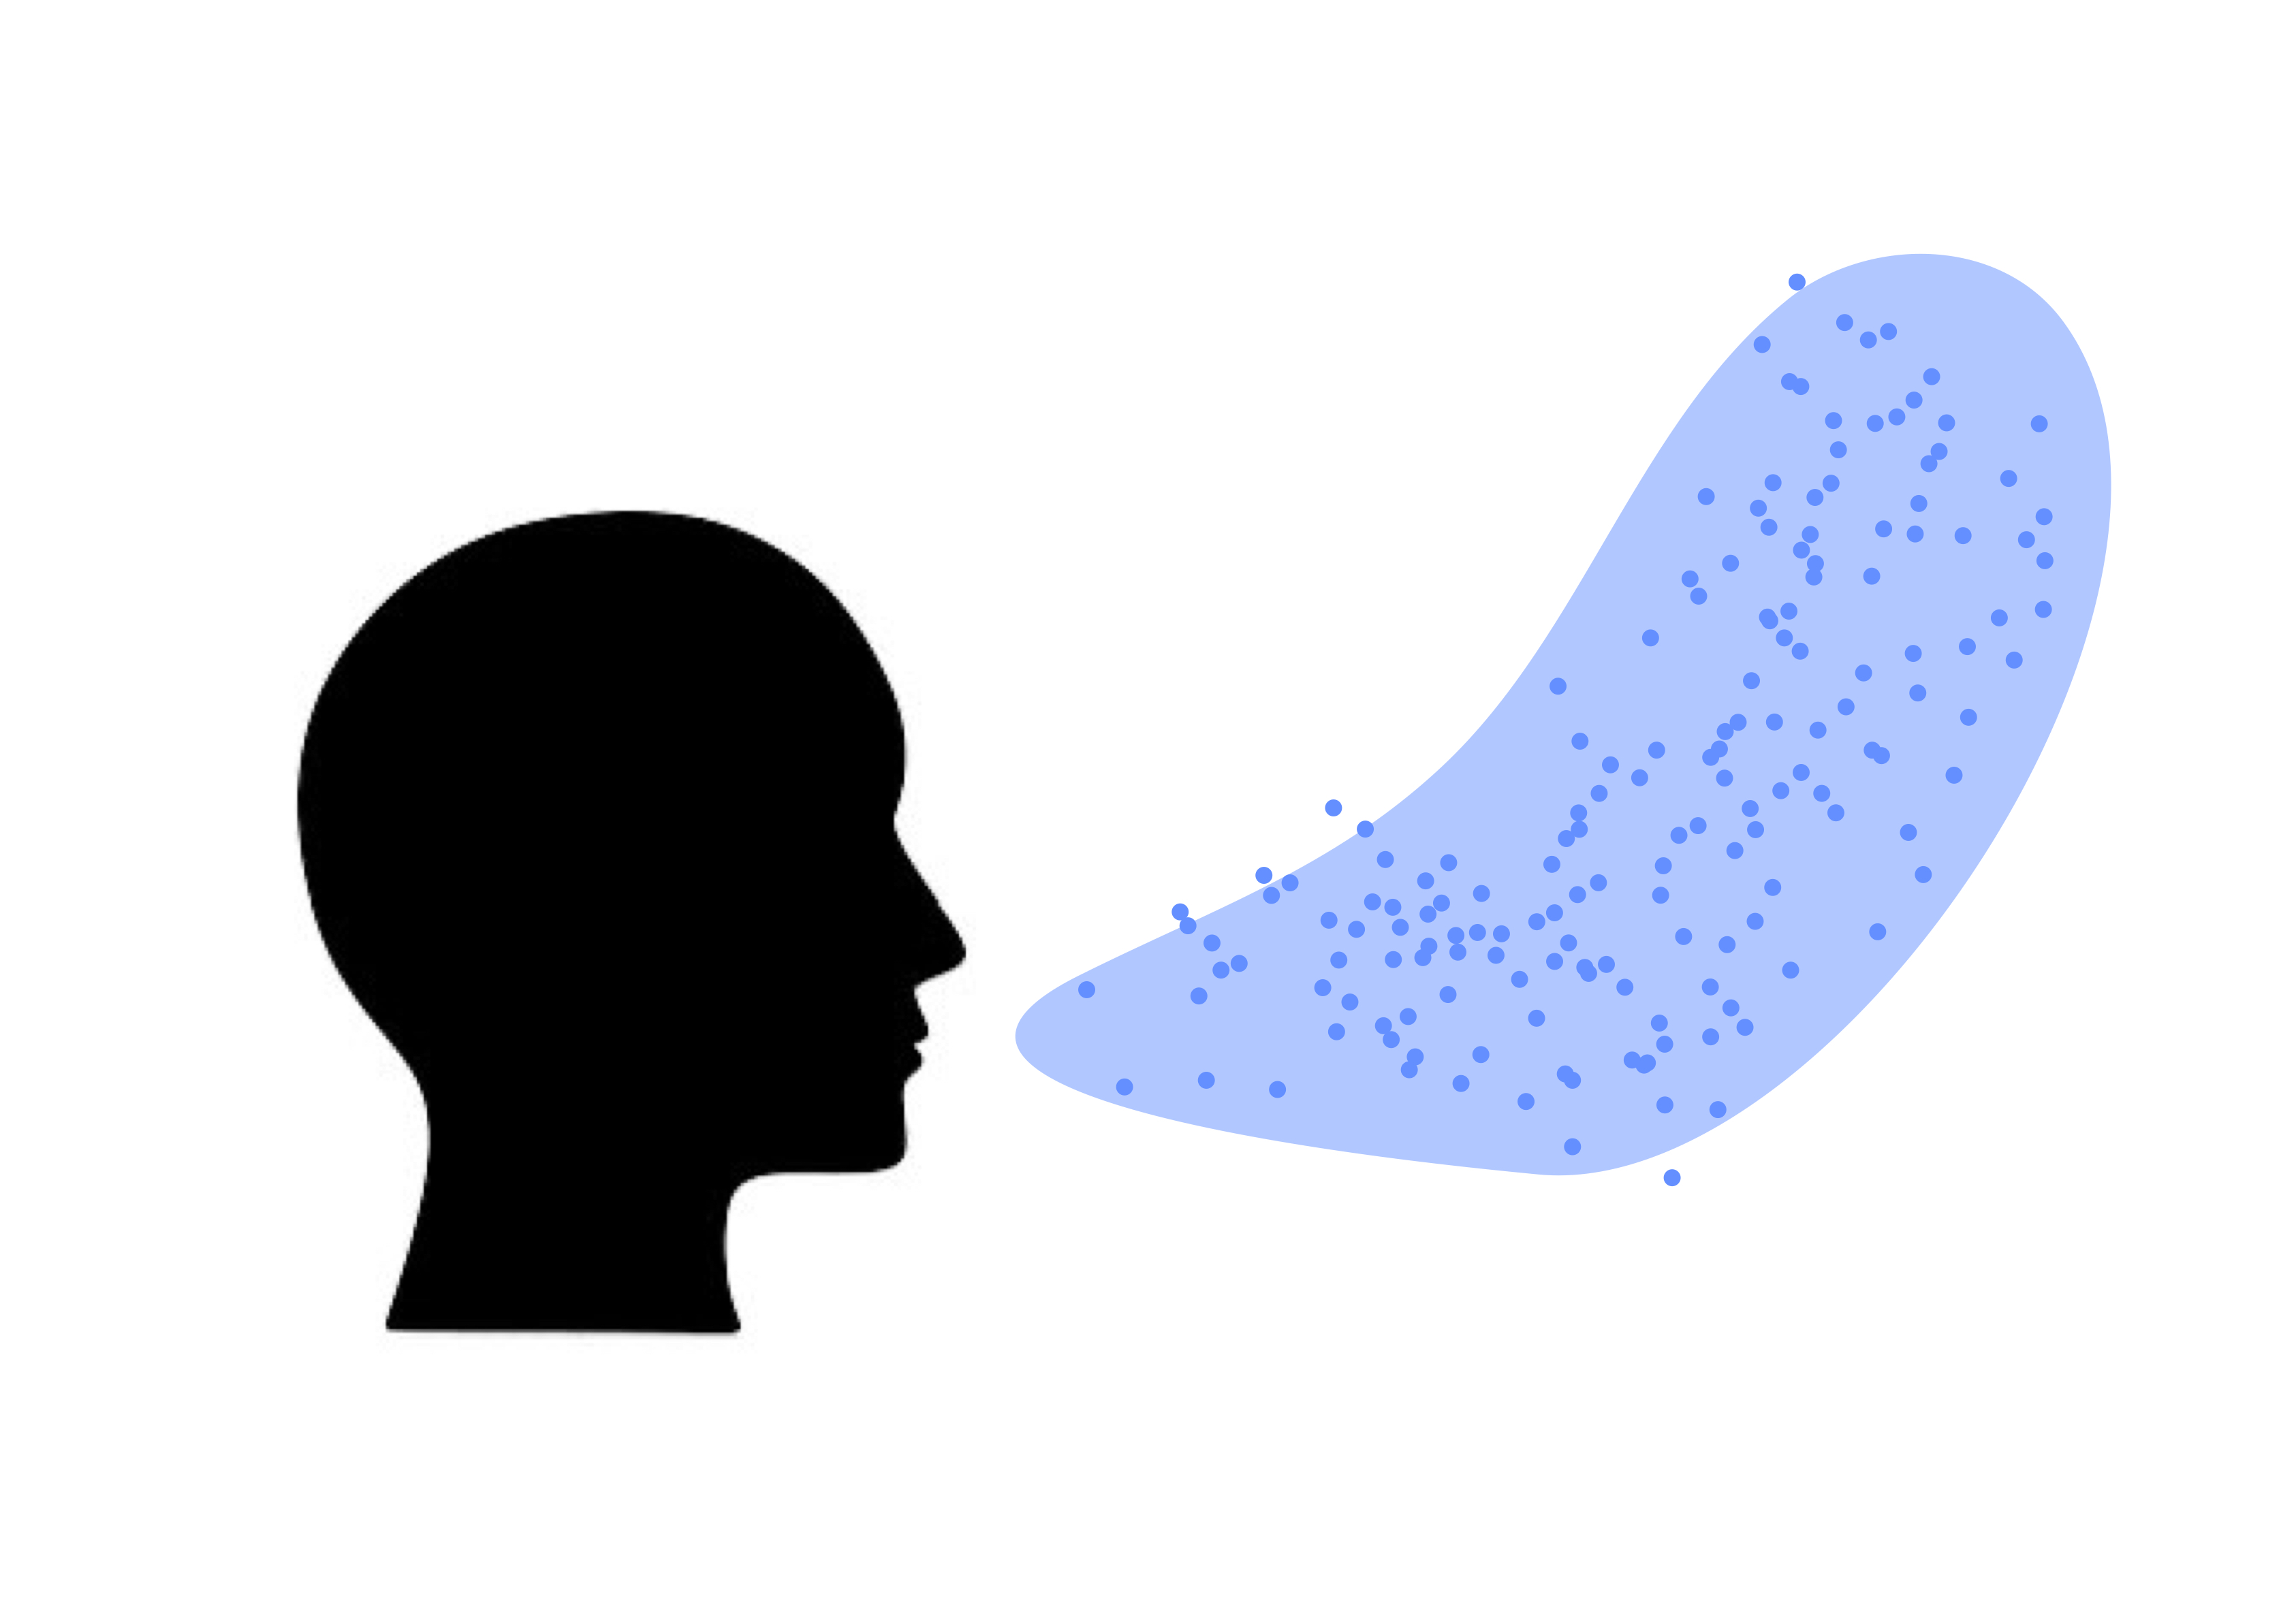
\includegraphics[clip,trim={0 2cm 0 2cm},width=0.25\textwidth]{Droplets/dropmat1.jpeg}& Coughing & 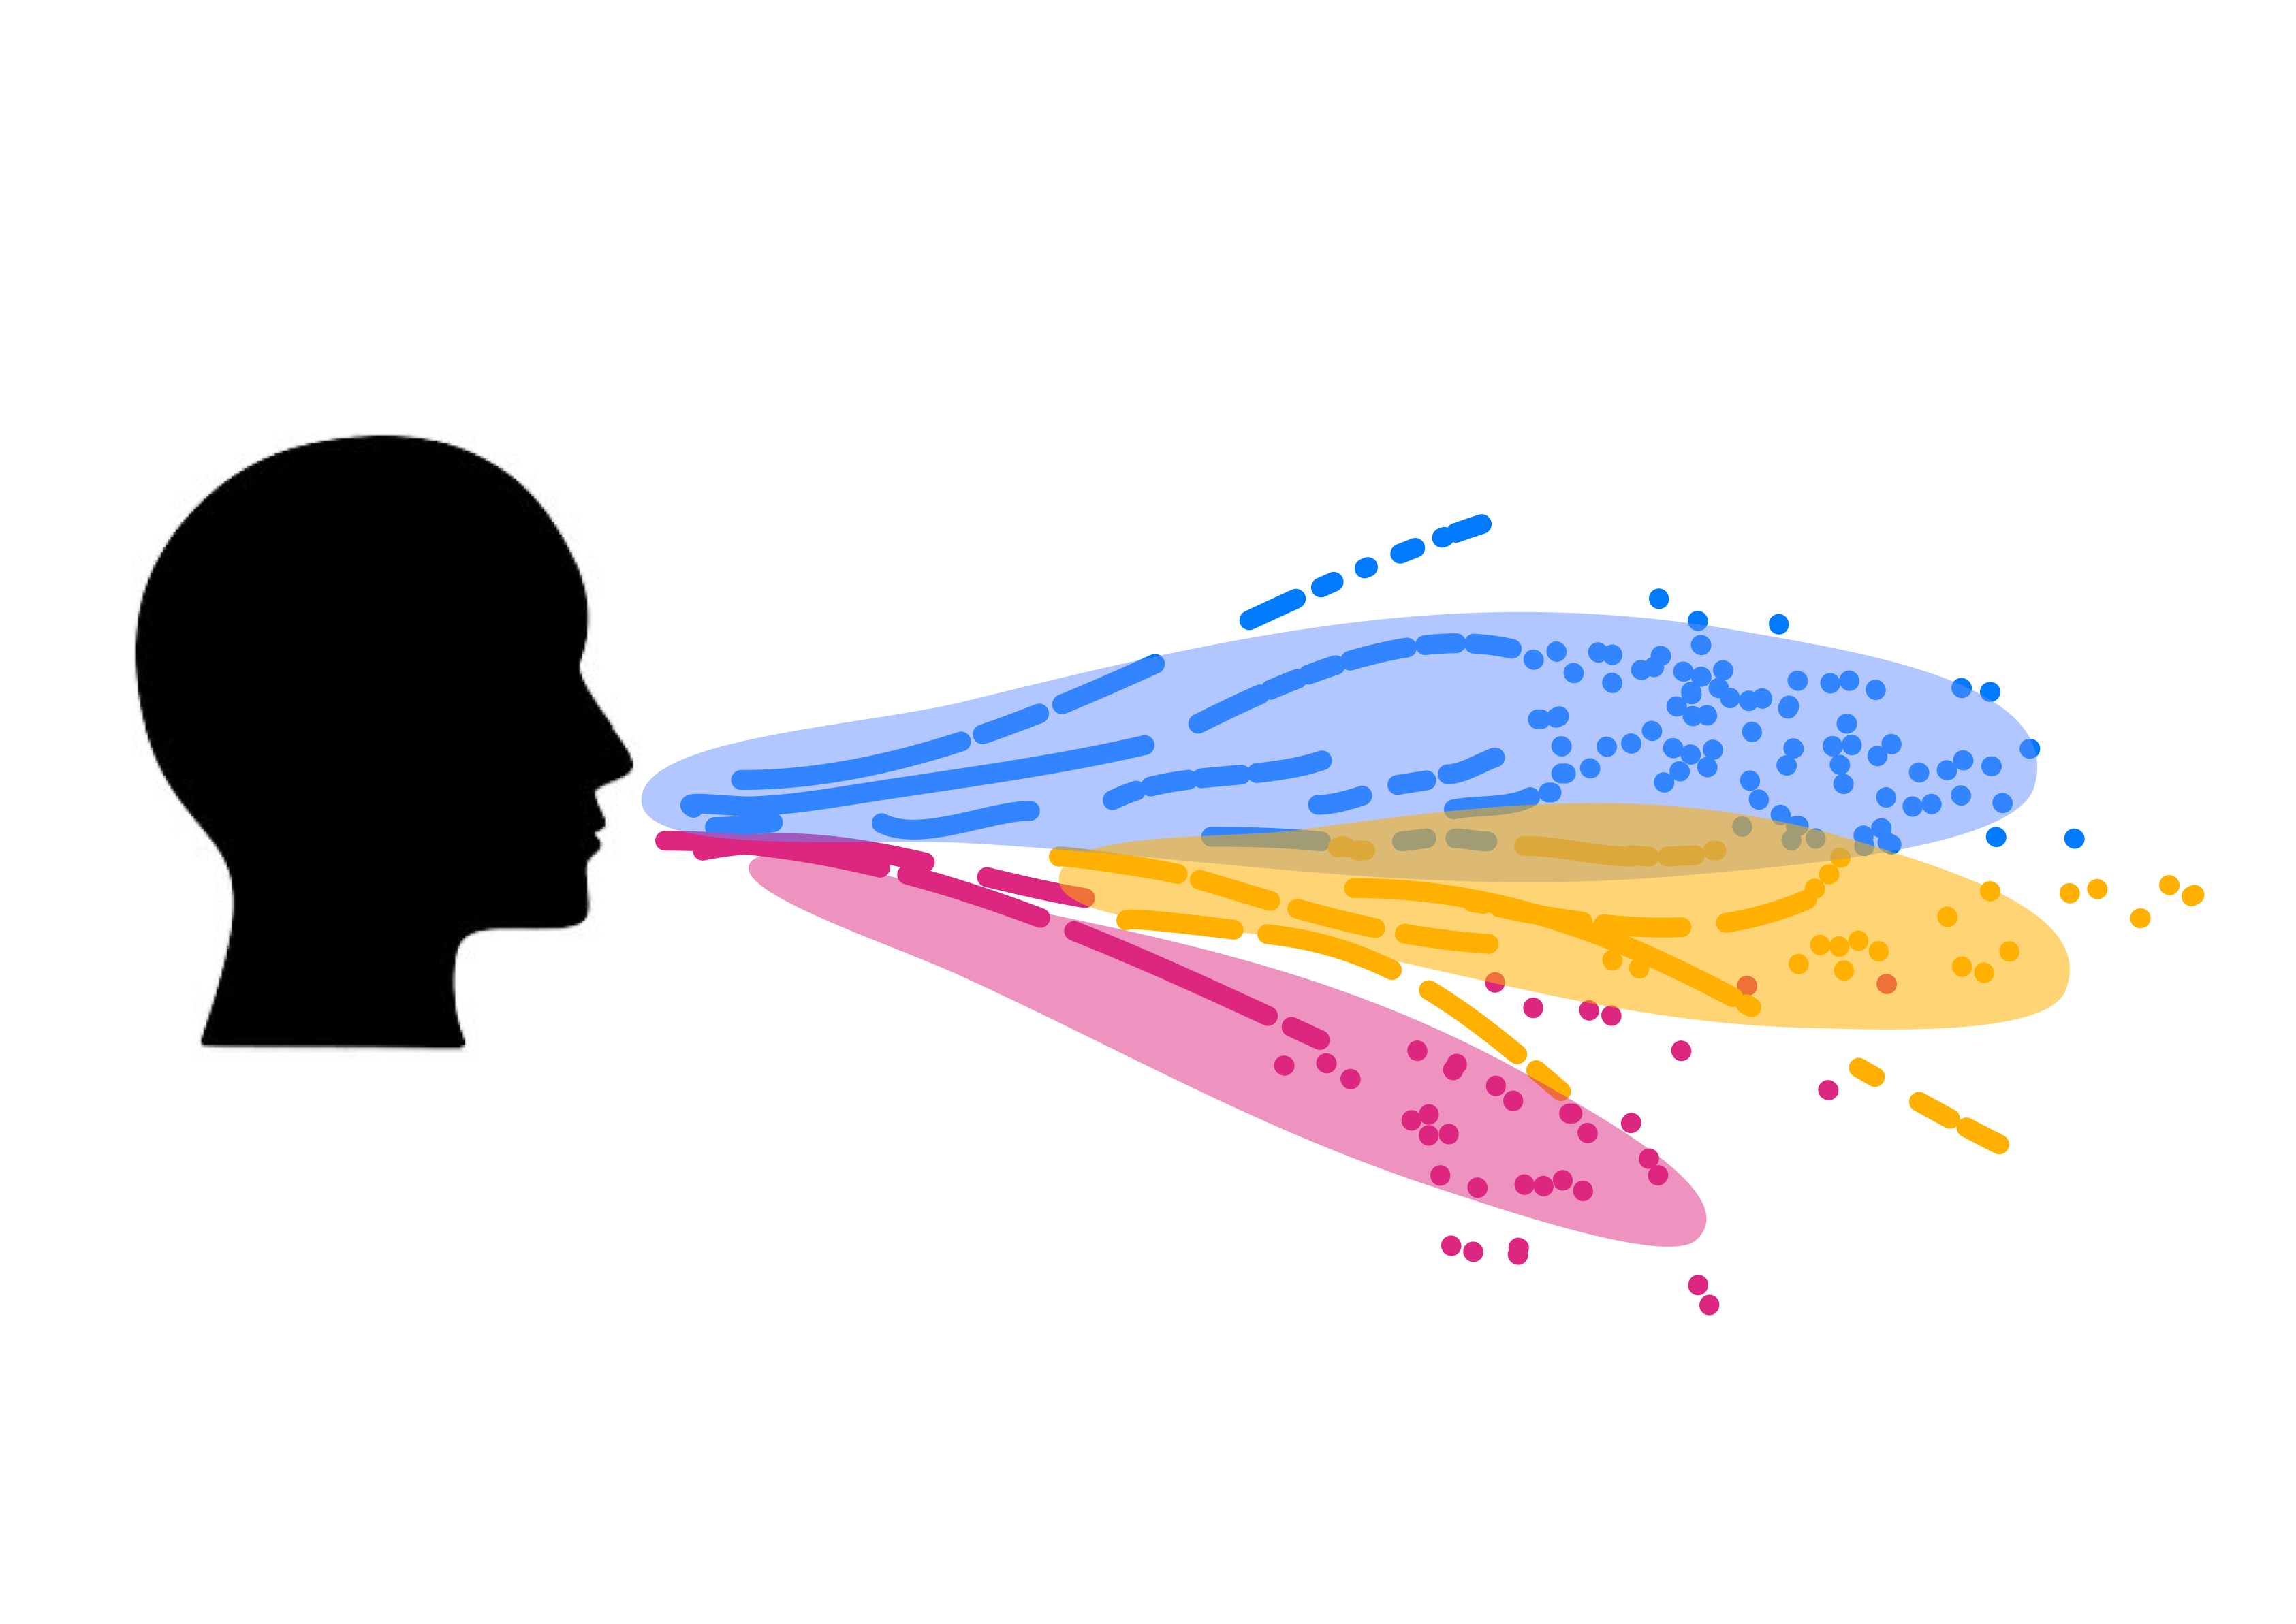
\includegraphics[clip,trim={0 2cm 0 2cm},width=0.25\textwidth]{Droplets/dropmat5.jpeg} \\
    \hline
    References & \cite{zhang2019distribution,feng2020study} & References & \cite{vuorinen2020modelling,diwan2020understanding,pendar2020numerical,lu2020reducing,rosti2020fluid,dbouk2020coughing,ren2021numerical,zhou2021experimental,sen2021transmission,mirzaie2021covid,chong2021extended,aliyu2021dispersion,yan2021transmission, lordly2022understanding,wang2022evaluation} \\
    \hline
    Low temperature \& High humidity & 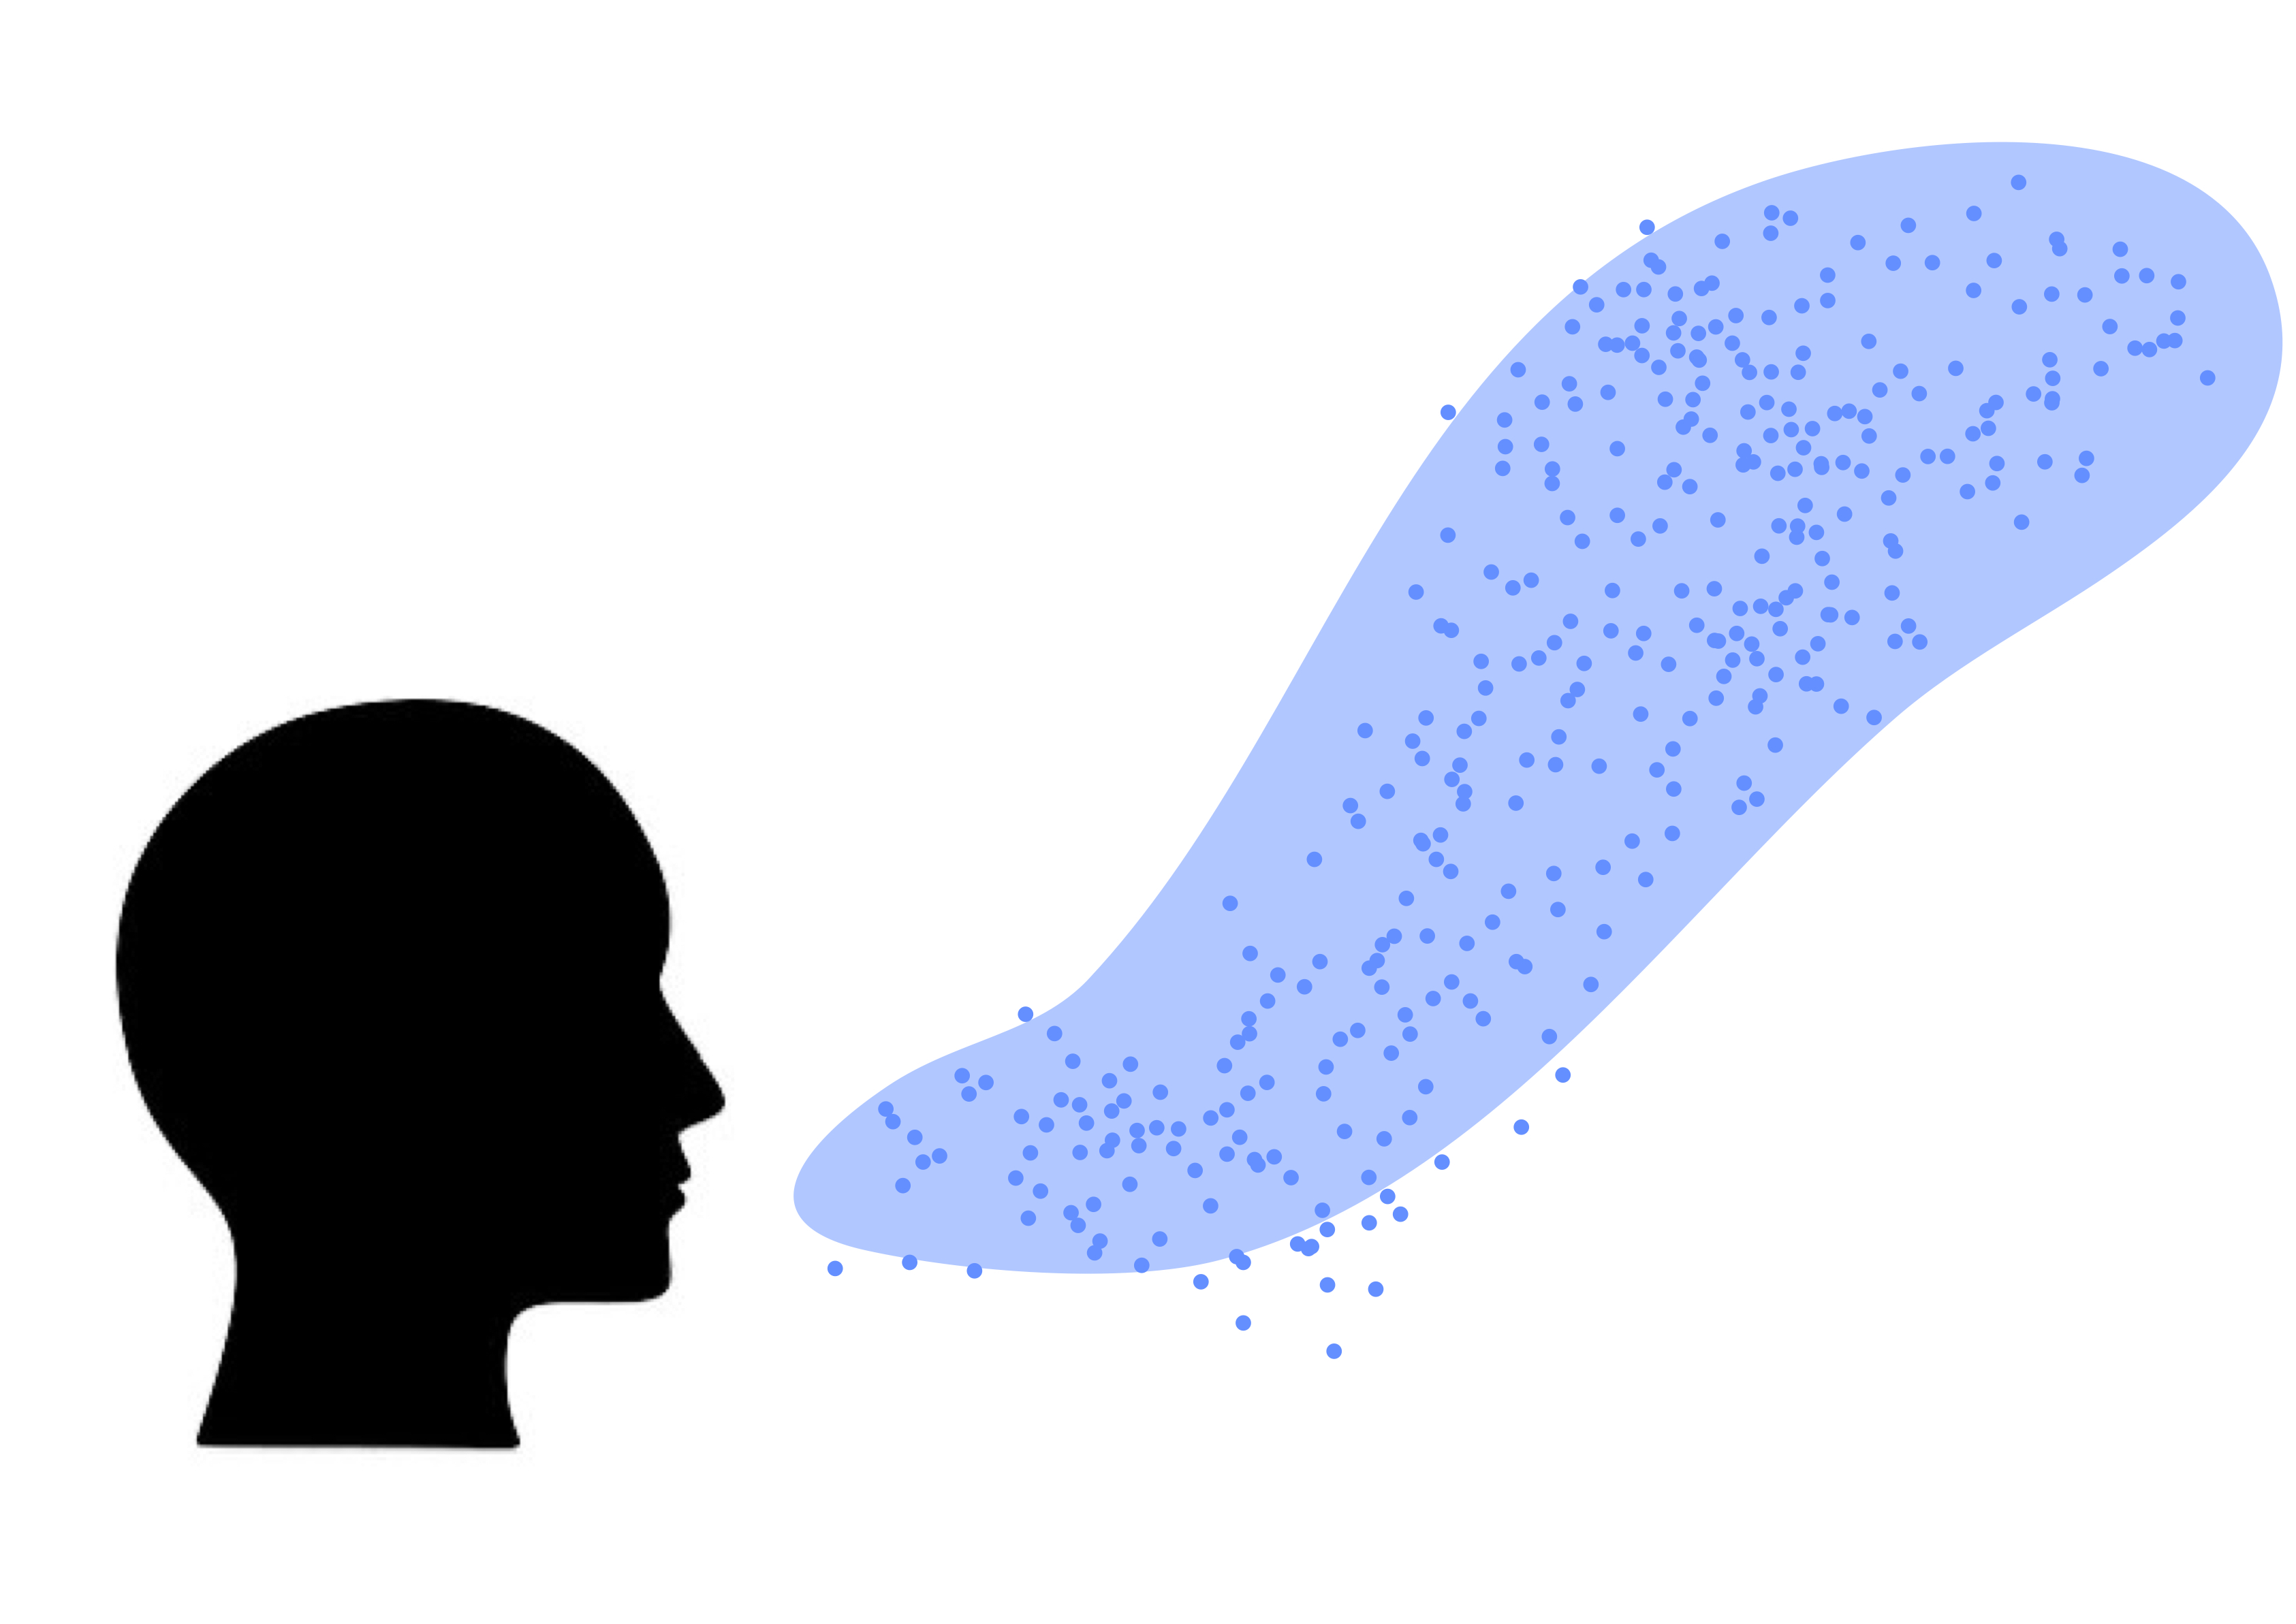
\includegraphics[clip,trim={0 2cm 0 2cm},width=0.25\textwidth]{Droplets/dropmat2.jpeg}& Sneezing & 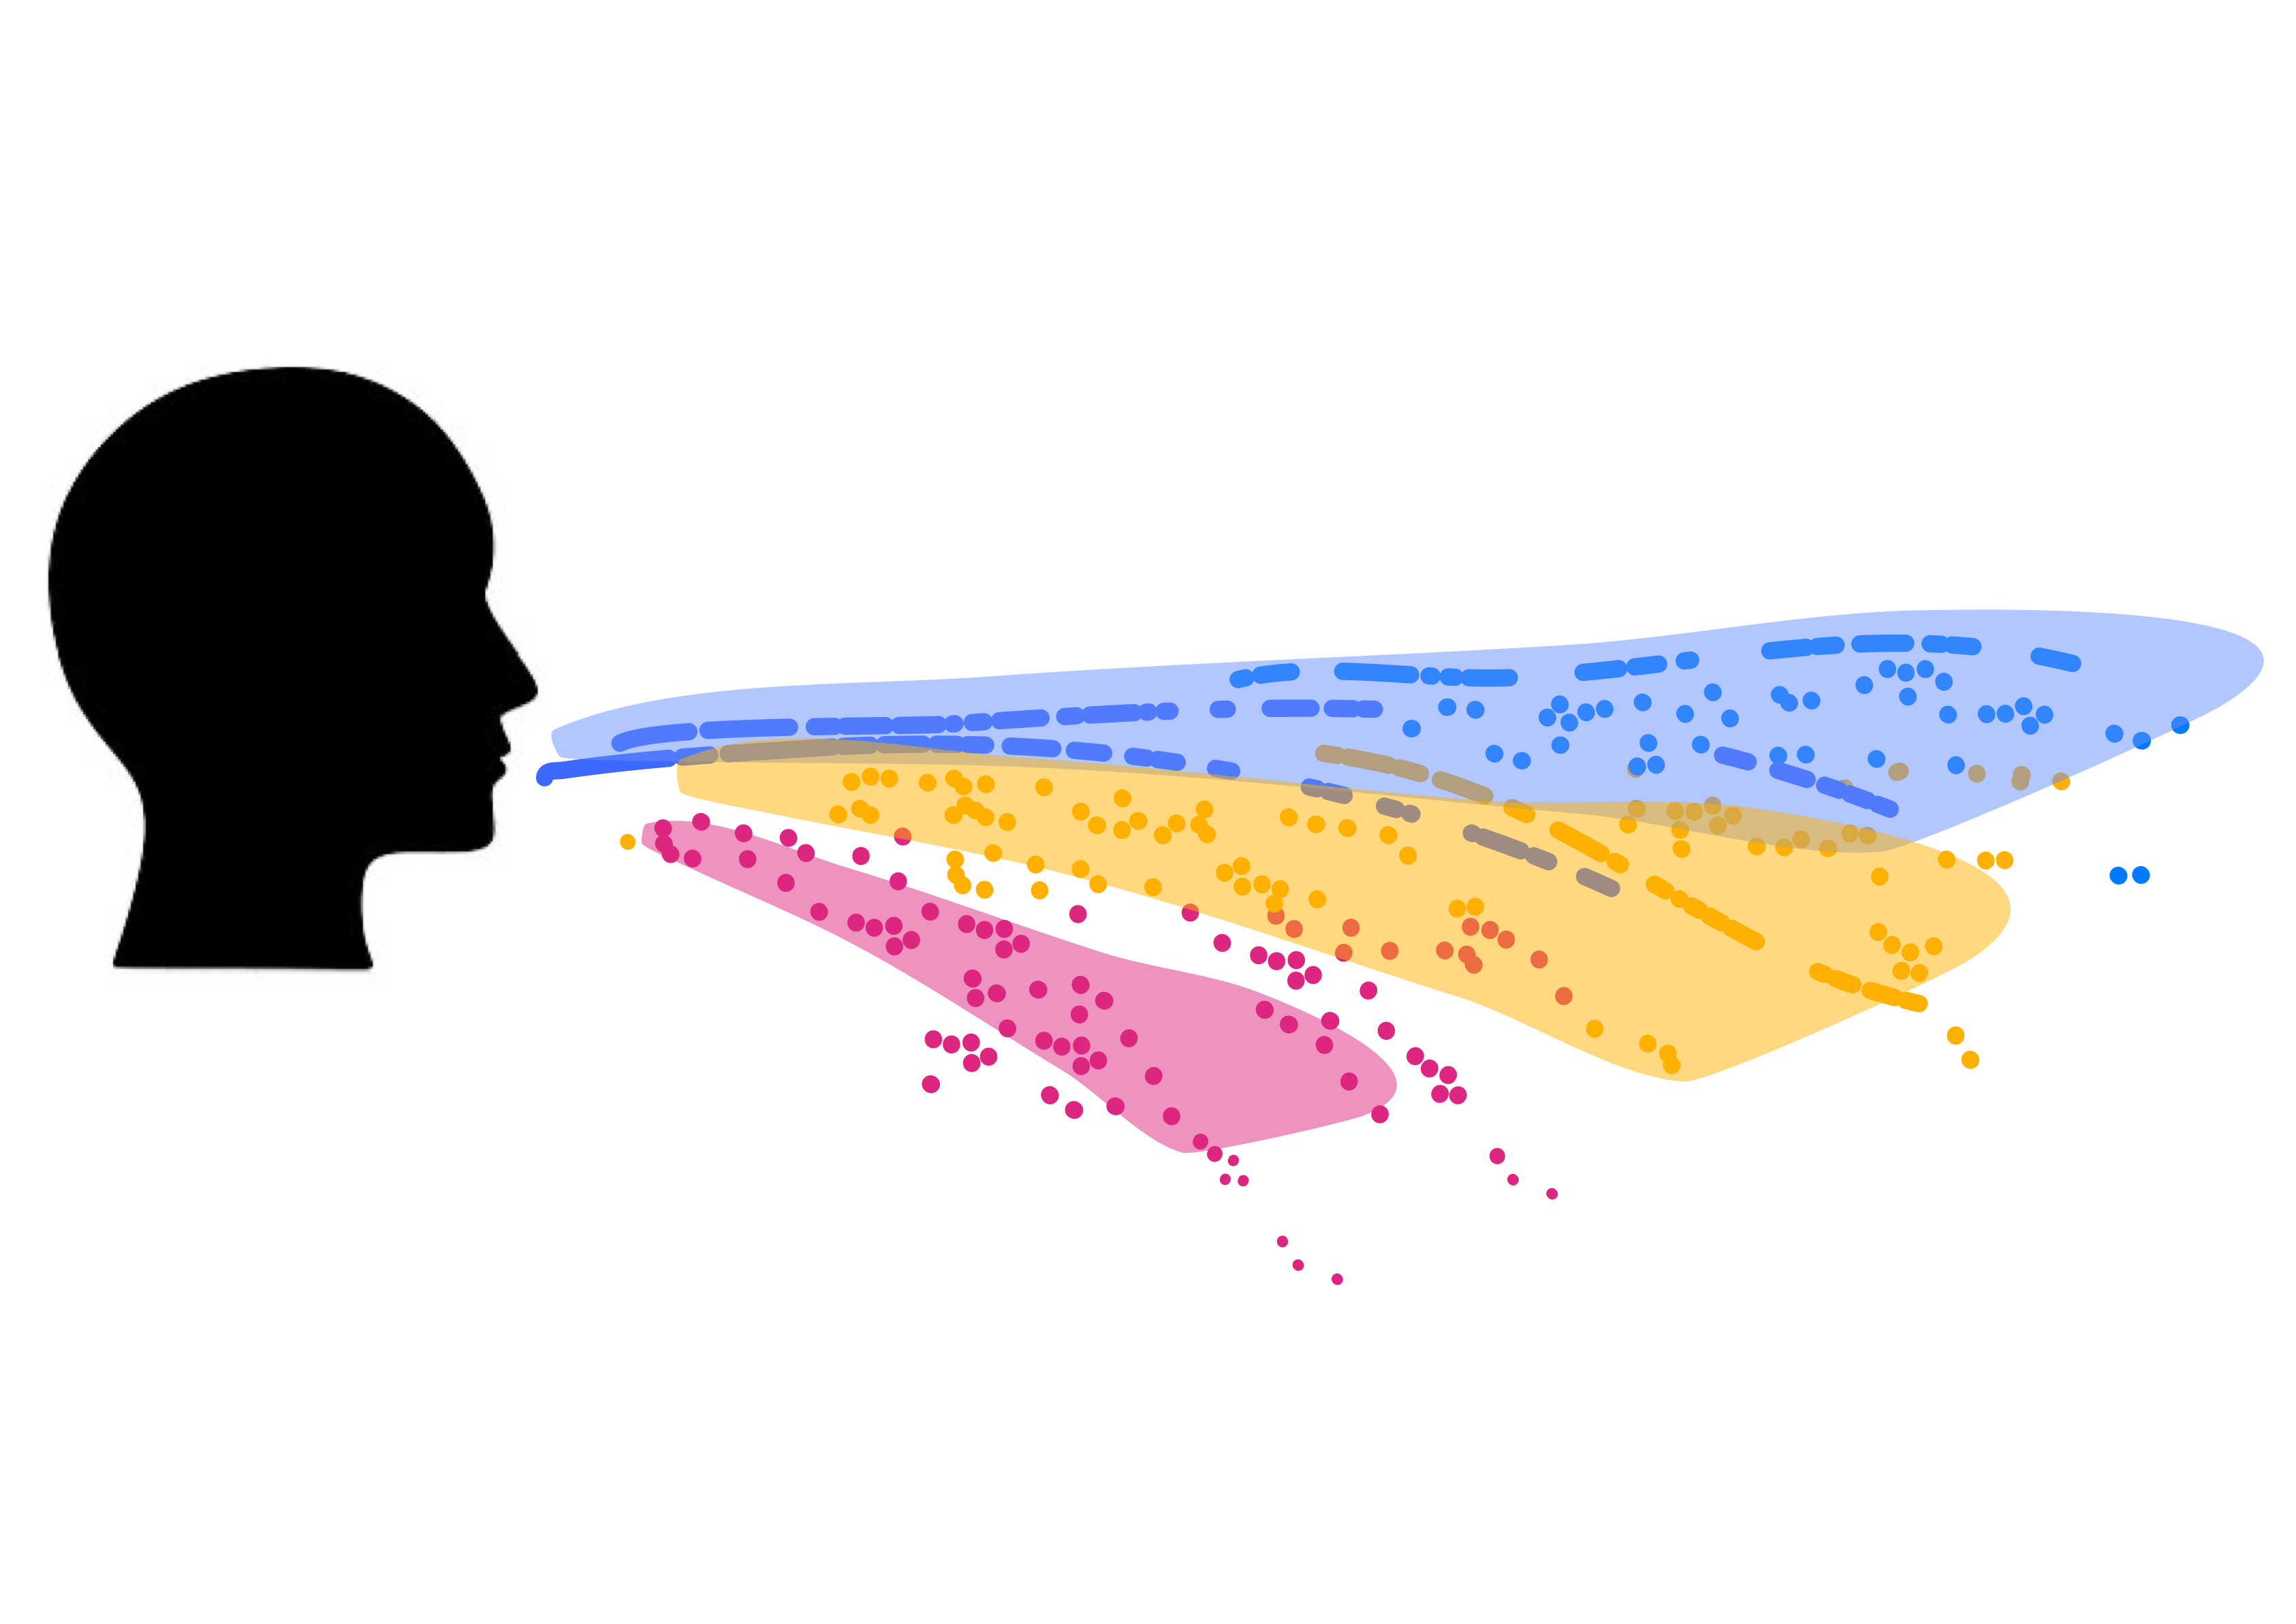
\includegraphics[clip,trim={0 2cm 0 2cm},width=0.25\textwidth]{Droplets/dropmat6.jpeg} \\
    \hline
    \textbf{References} & \cite{zhang2019distribution,chong2021extended} & \textbf{References} & \cite{pendar2020numerical,diwan2020understanding,fontes2020study,aliyu2021dispersion} \\
    \hline
    High temperature \& Low humidity & 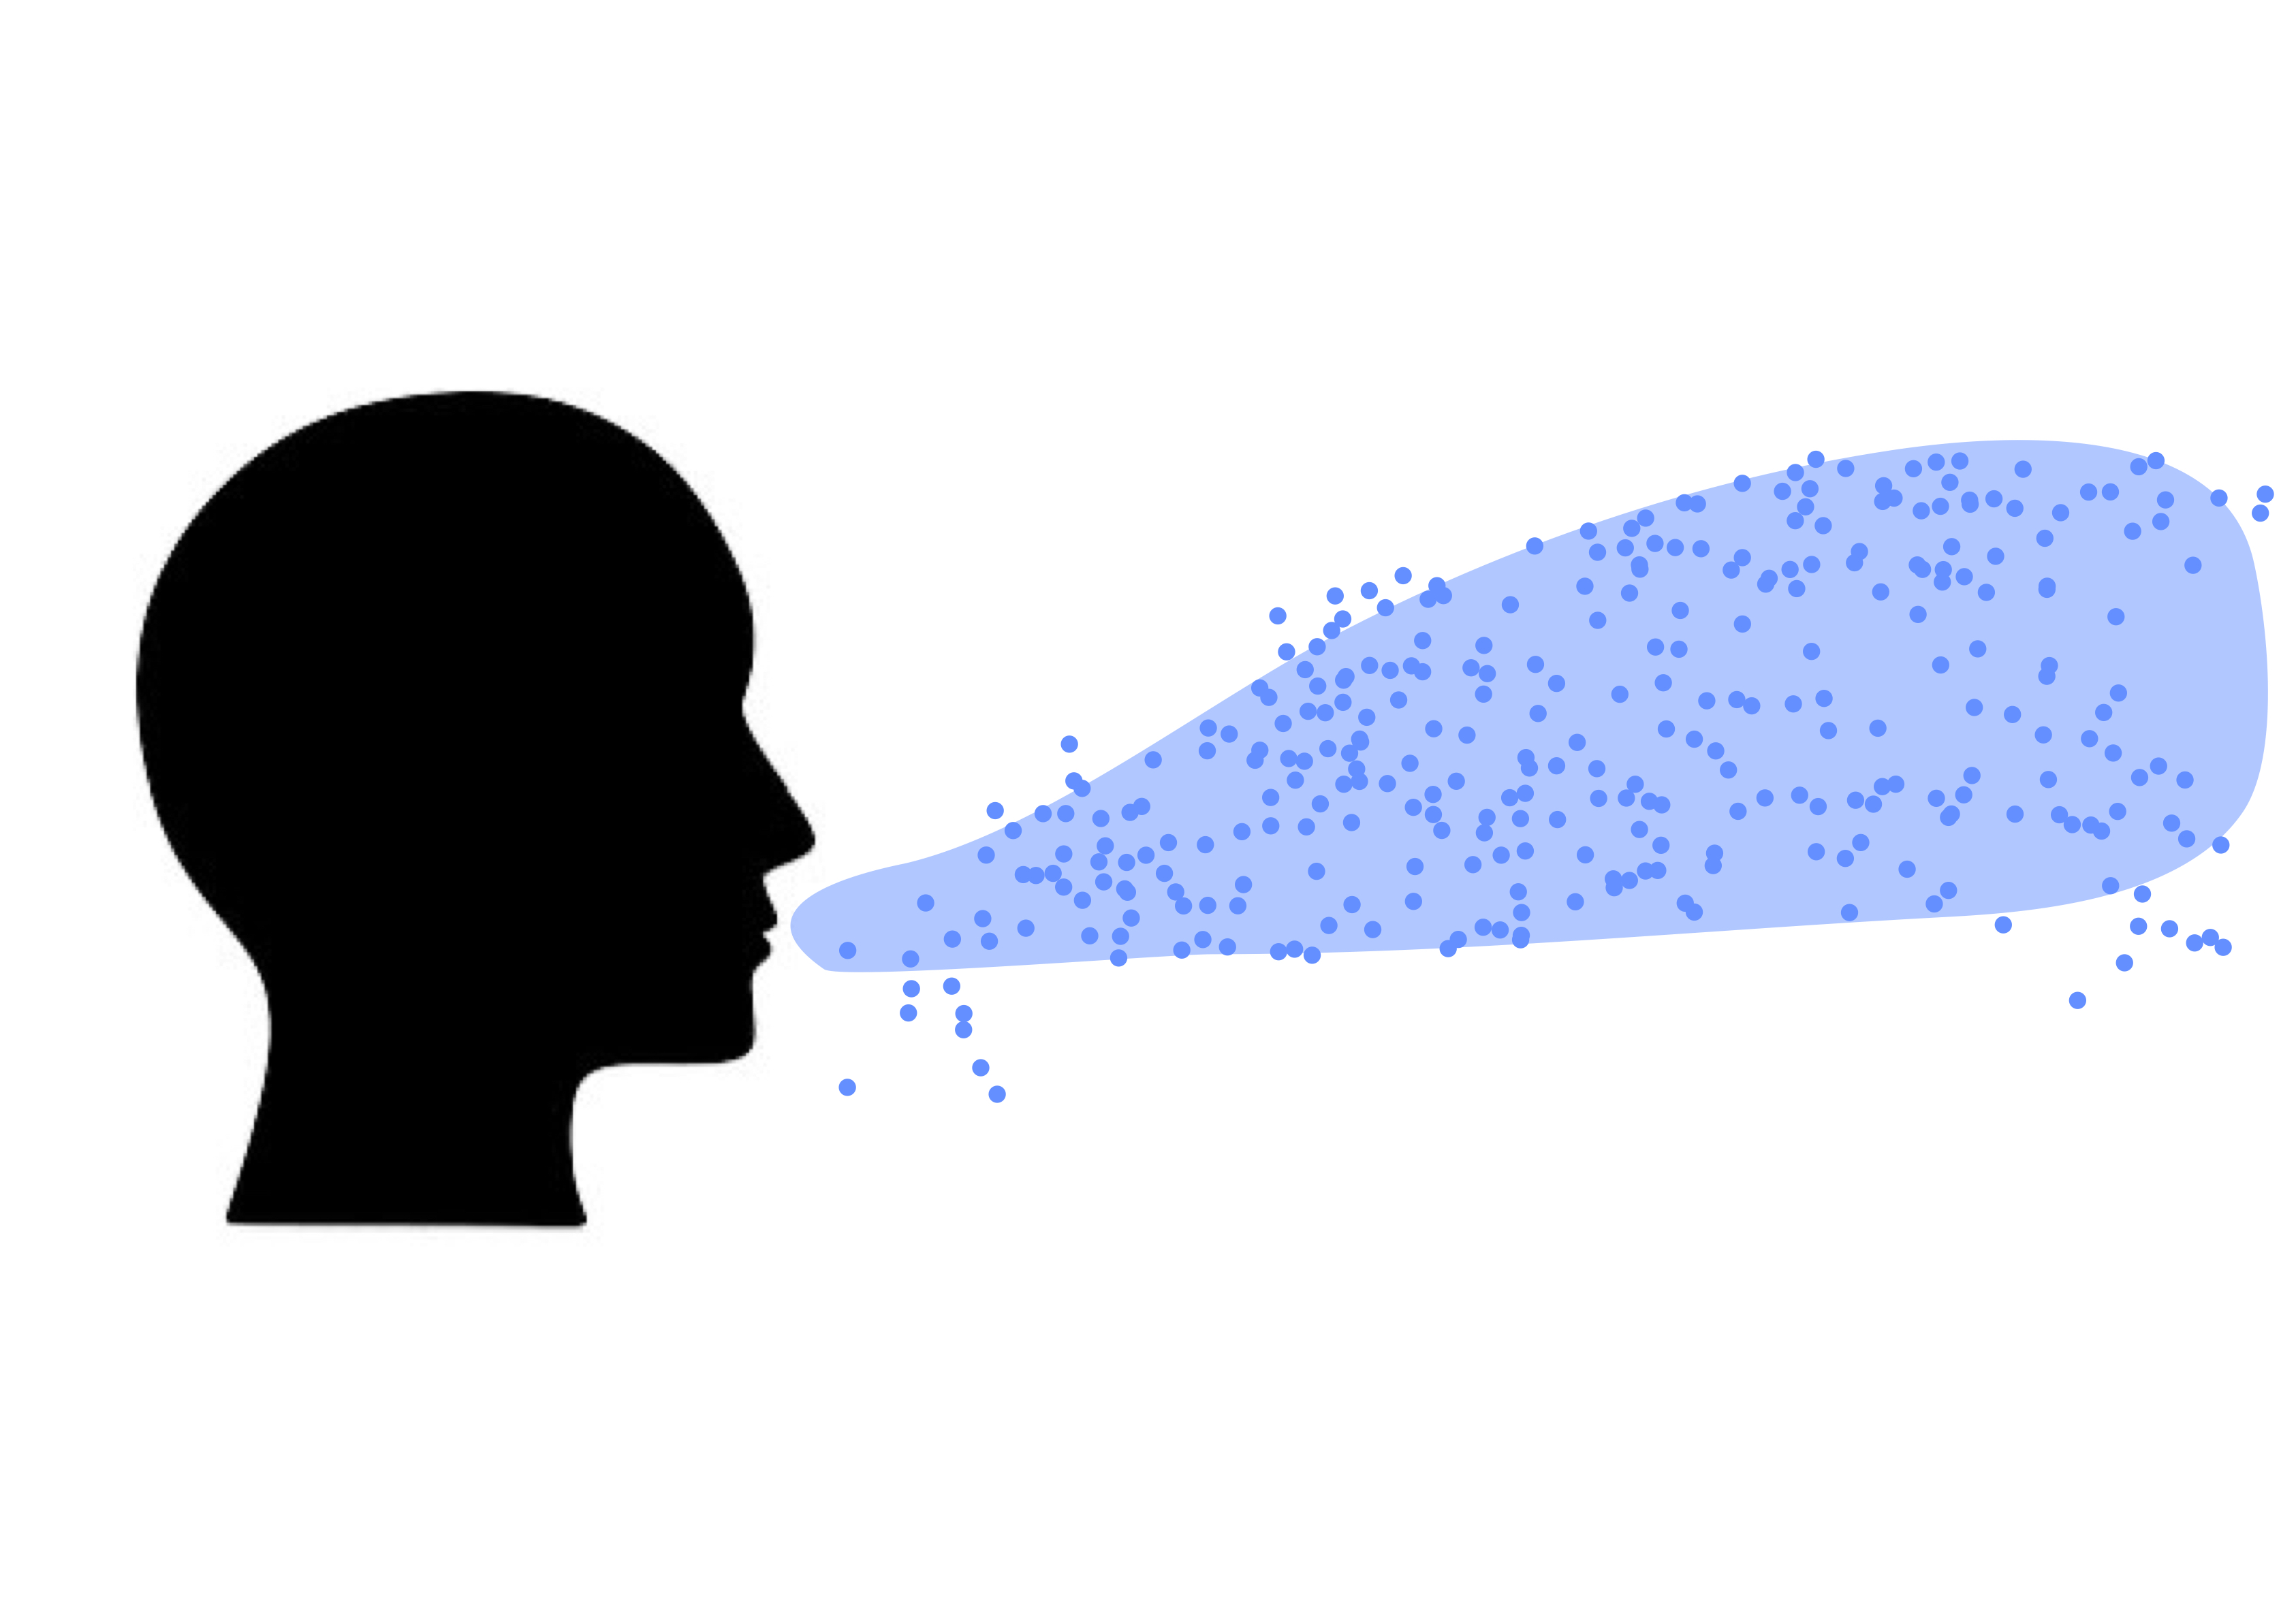
\includegraphics[clip,trim={0 2cm 0 2cm},width=0.25\textwidth]{Droplets/dropmat3.jpeg}& Breathing & 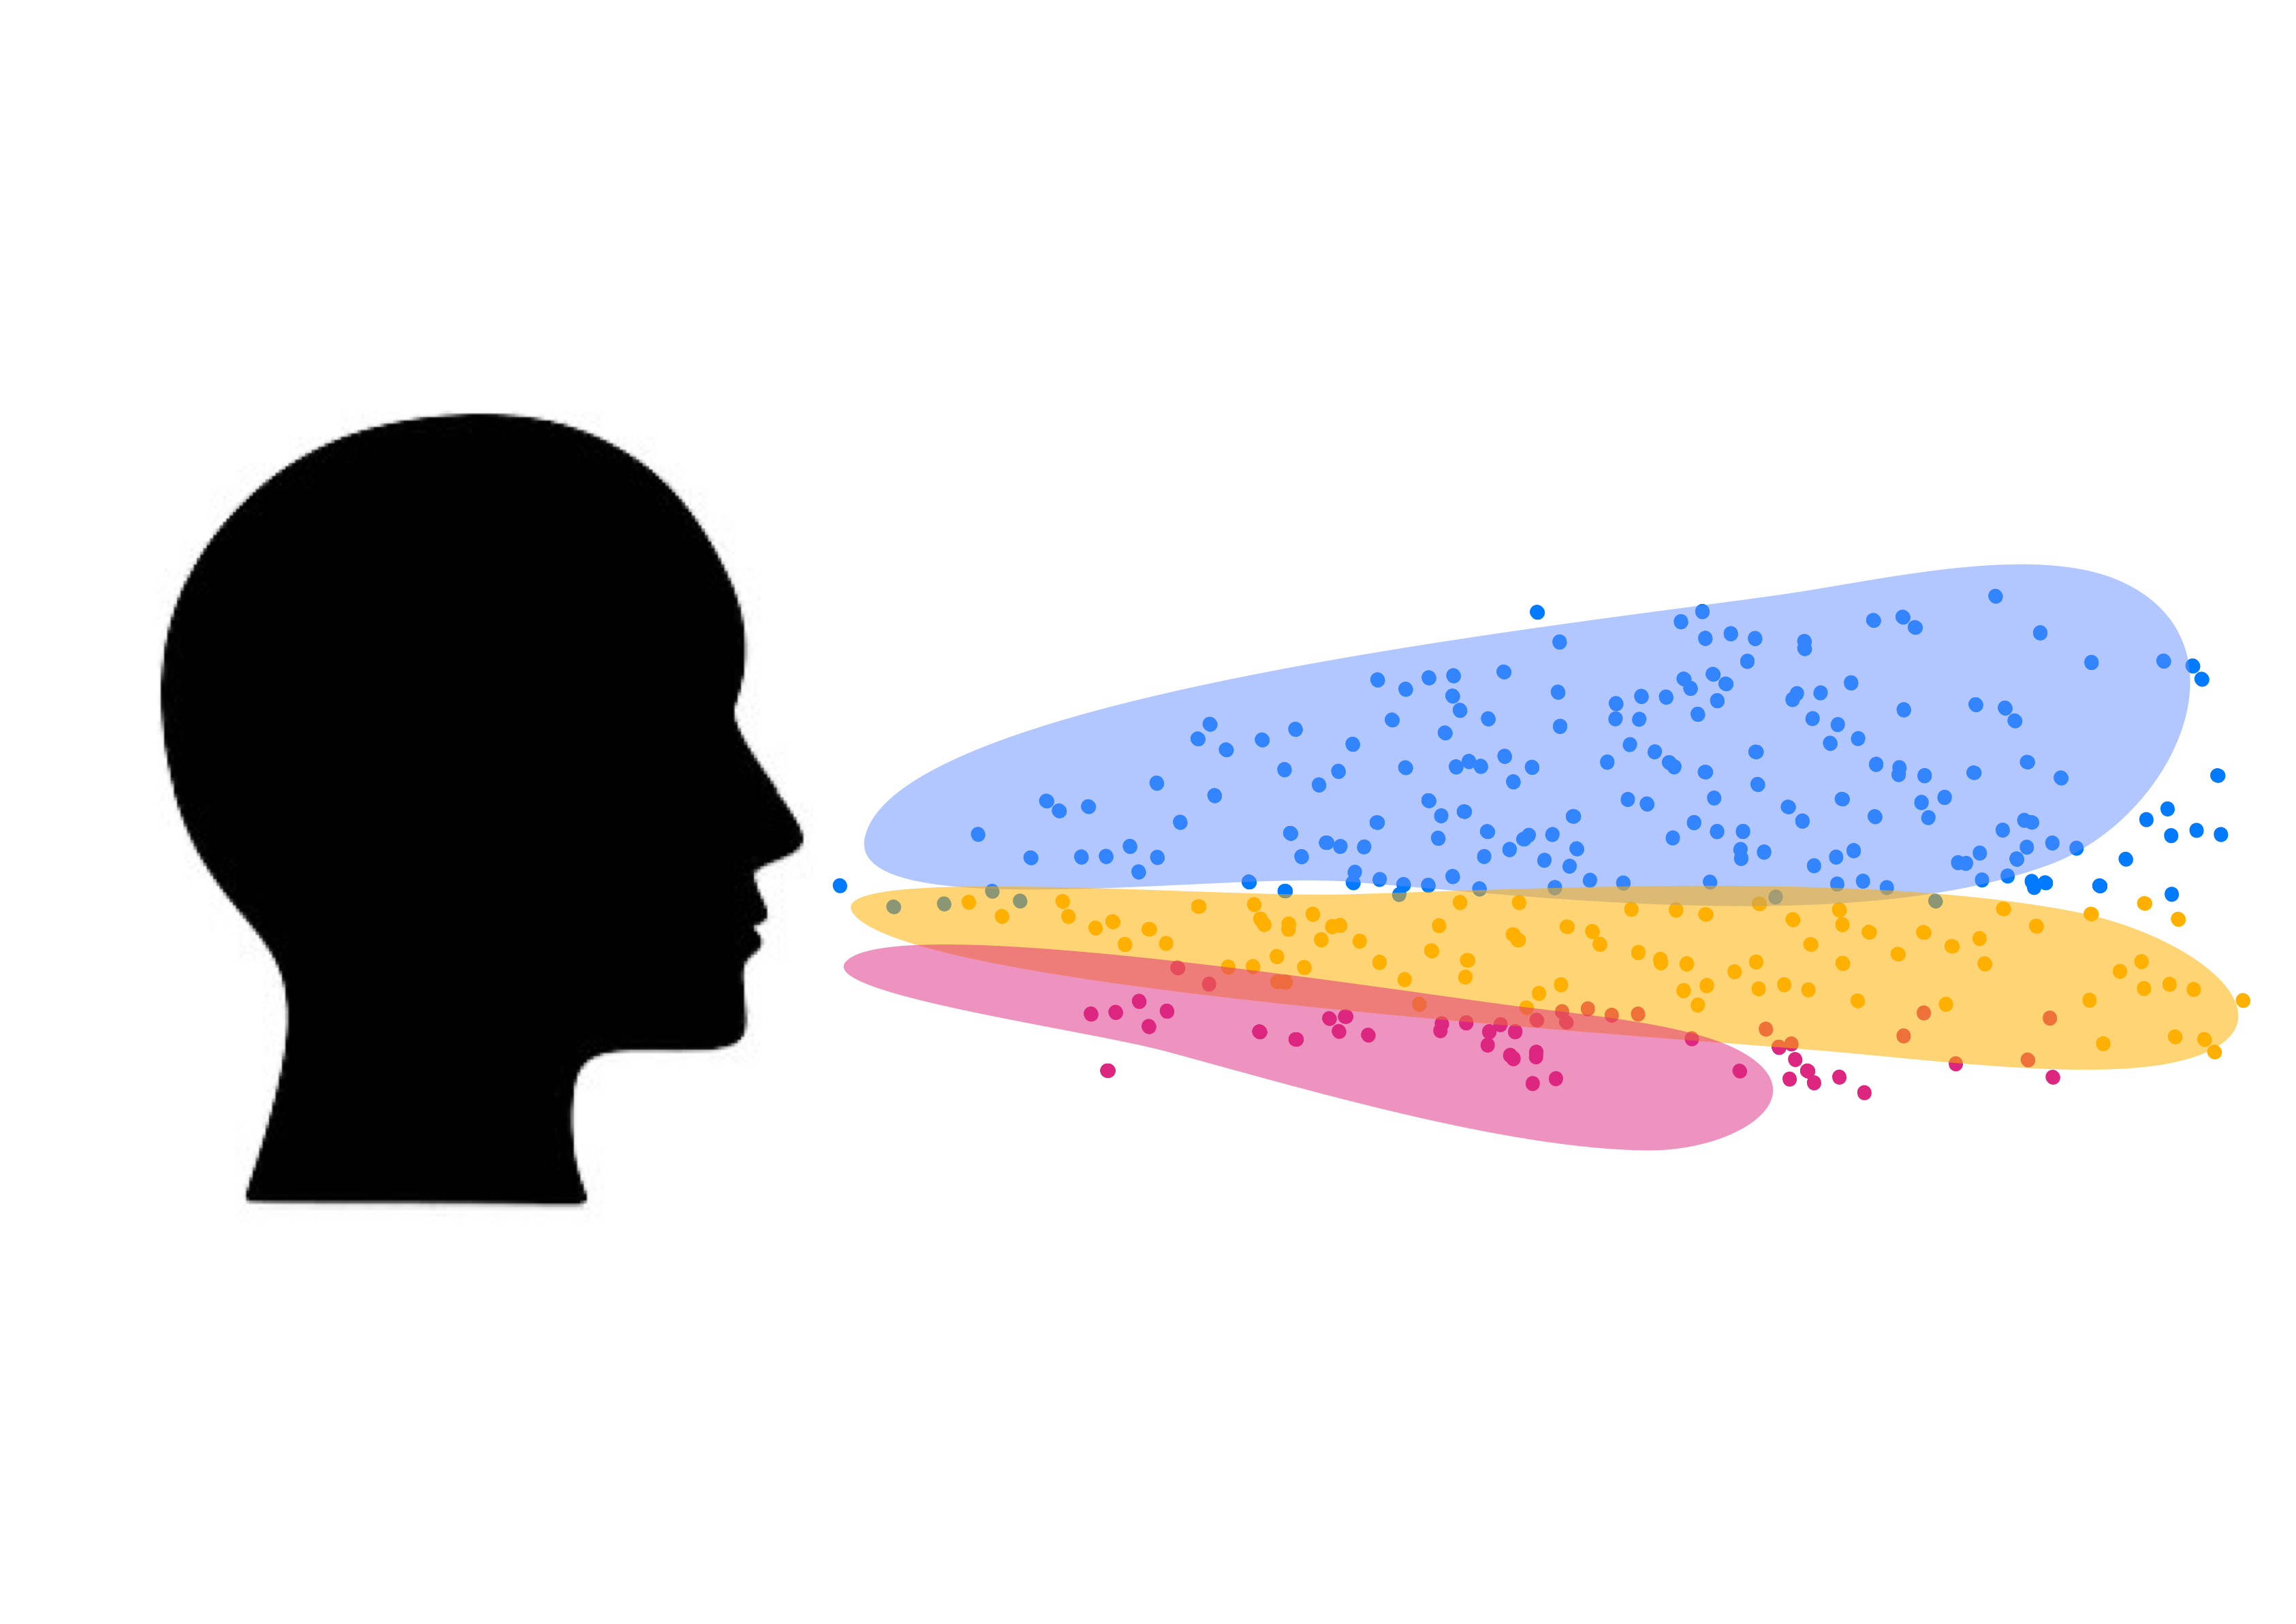
\includegraphics[clip,trim={0 2cm 0 2cm},width=0.25\textwidth]{Droplets/dropmat7.jpeg} \\
    \hline
    \textbf{References} & \cite{zhang2019distribution,feng2020study,sen2021transmission} & \textbf{References} & \cite{he2011cfd,villafruela2019assessment,duill2021impact,shao2021risk,luo2022role,wang2022evaluation,wei2023effects} \\
    \hline
   High temperature \& High humidity & 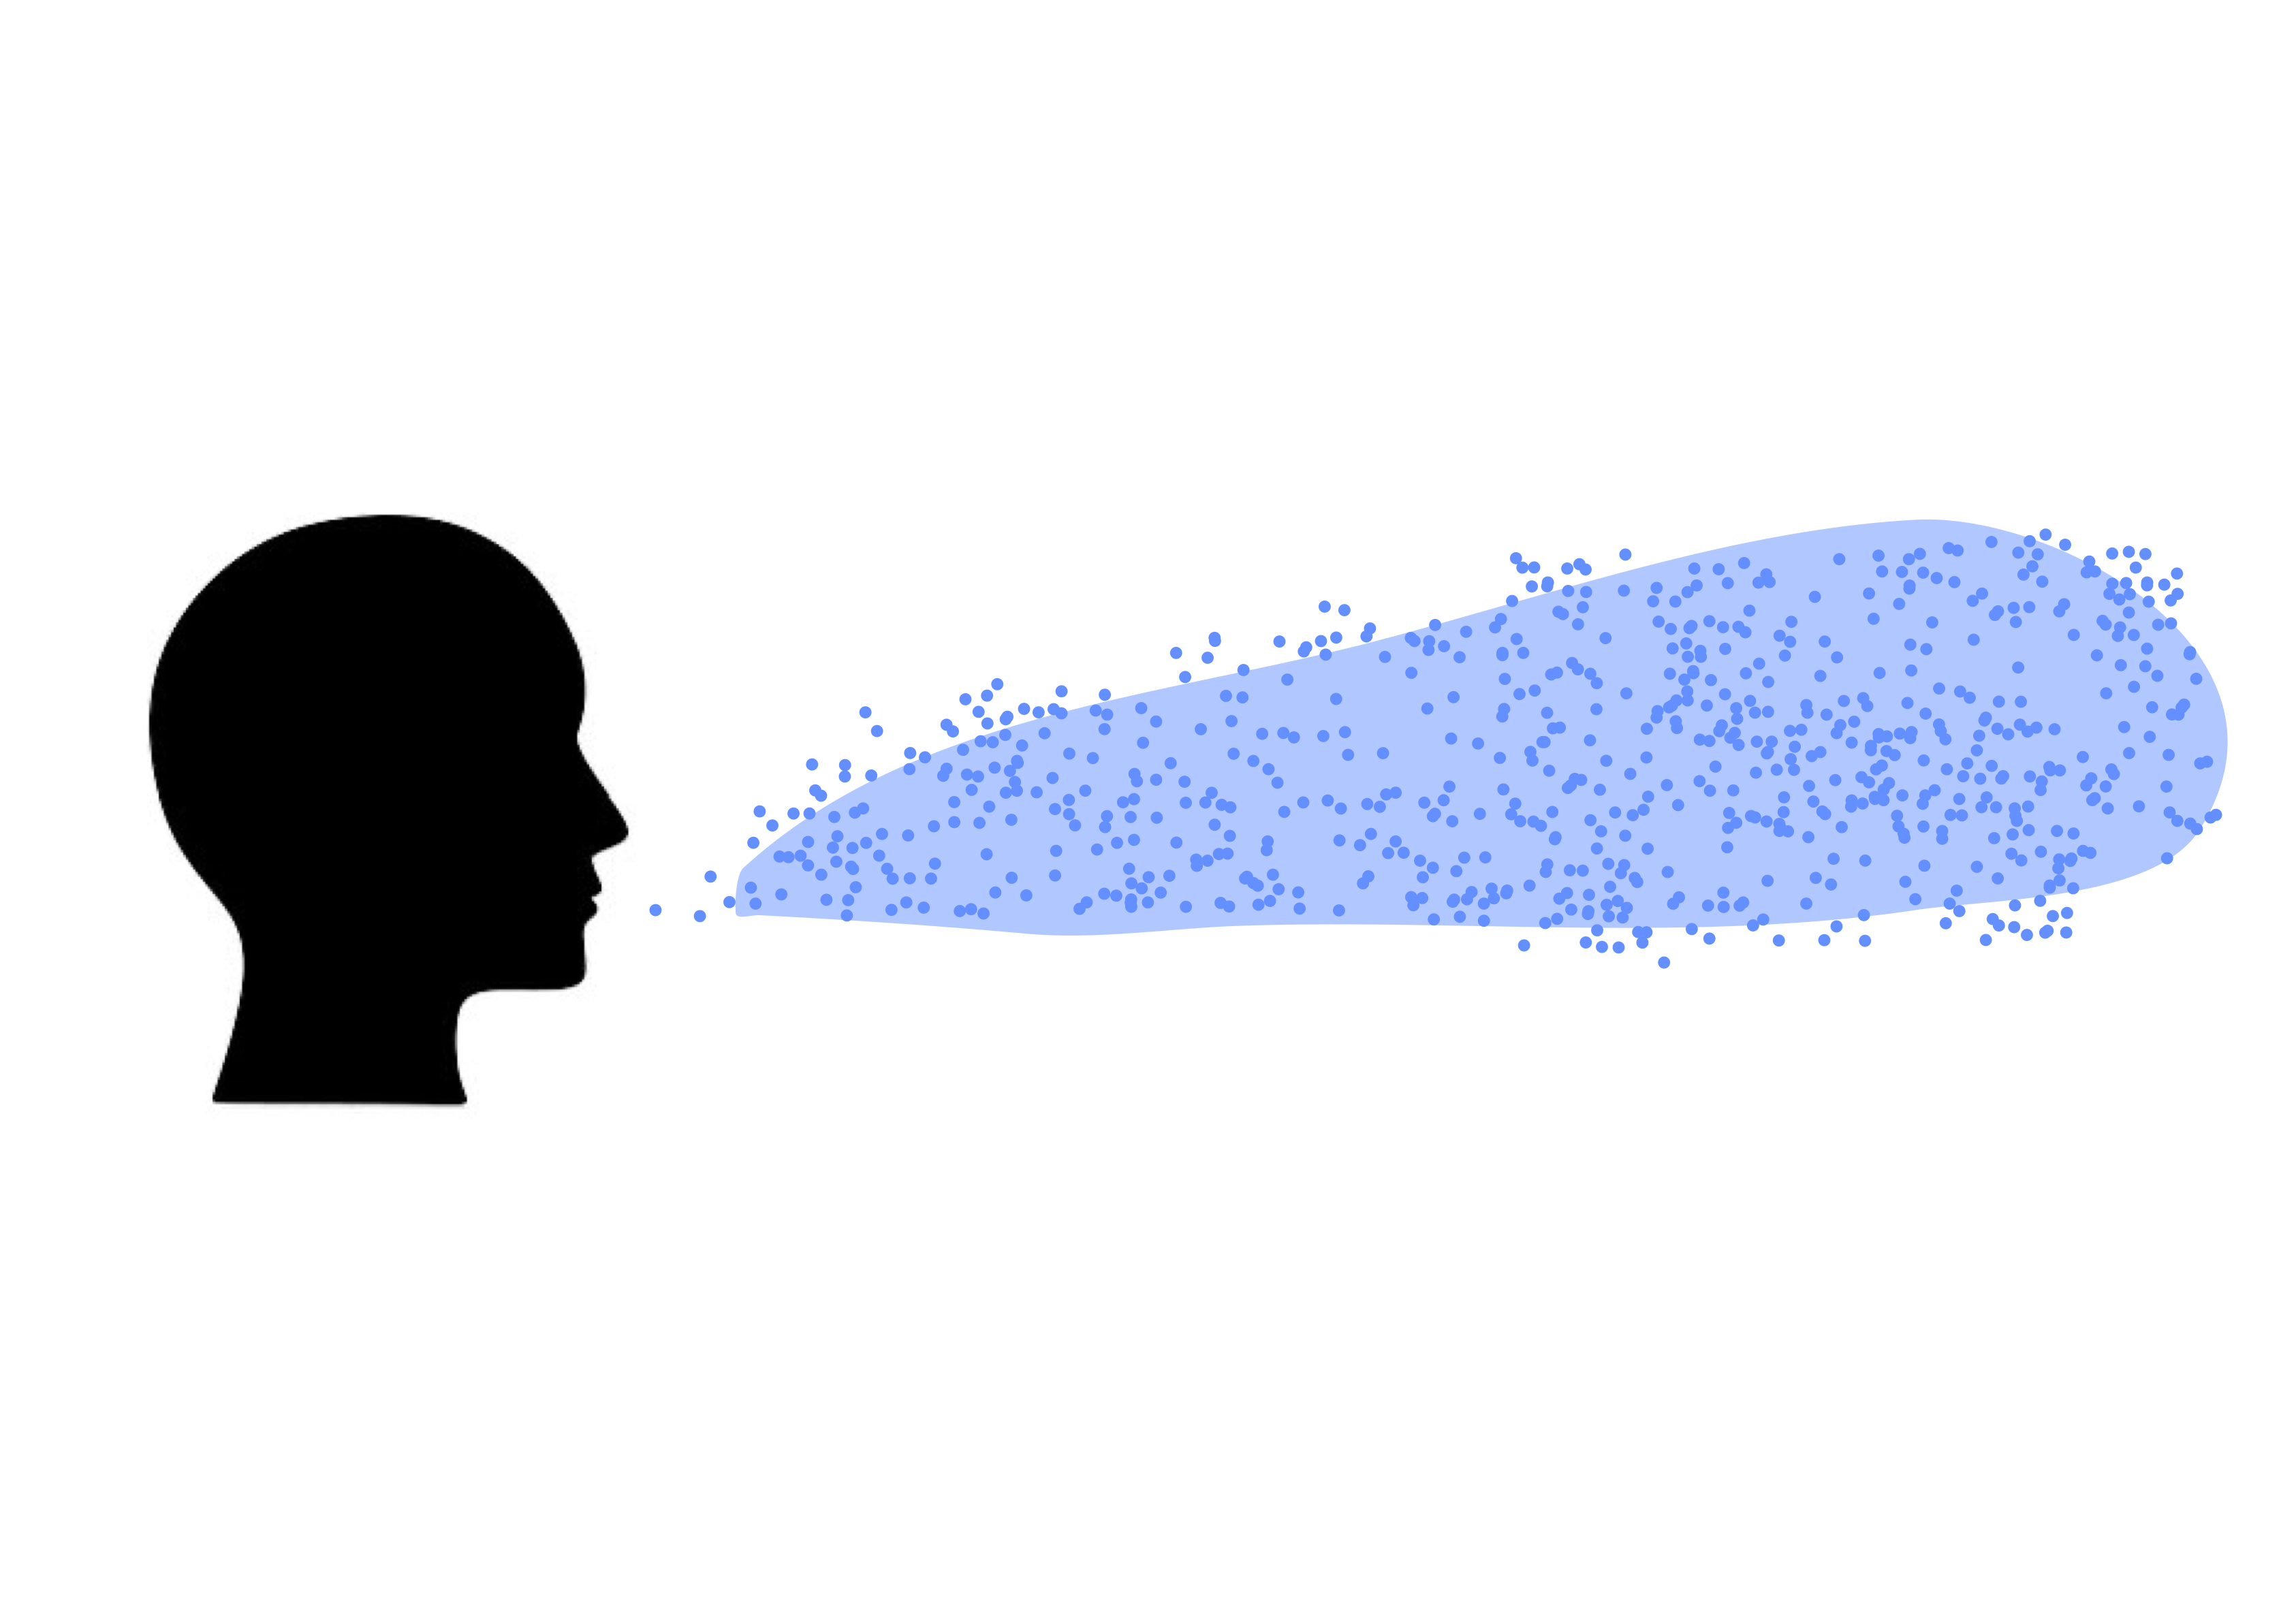
\includegraphics[clip,trim={0 2cm 0 2cm},width=0.25\textwidth]{Droplets/dropmat4.jpeg}& Speaking & 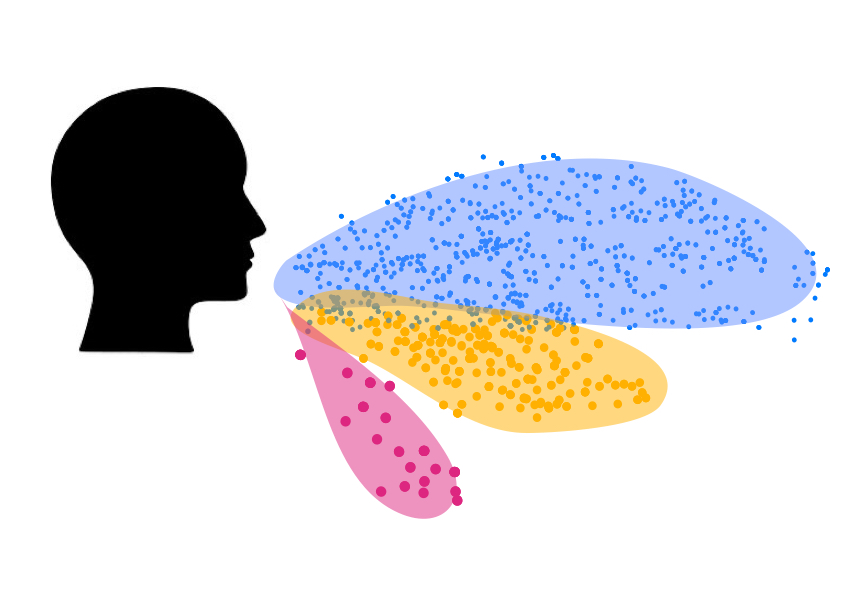
\includegraphics[clip,trim={0 2cm 0 2cm},width=0.25\textwidth]{Droplets/dropmat8.jpeg} \\
    \hline
    \textbf{References} & \cite{zhang2019distribution,chong2021extended} & \textbf{References} & \cite{vuorinen2020modelling,zhou2021experimental,wang2022evaluation,wei2023effects} \\
    \hline
    \end{tabular}
    \caption{Schematics of droplet plumes in different ambient conditions and respiratory activity. The different-sized droplets expelled during different respiratory activities are shown as: \legendsquare{fill=resp} Small droplets \legendsquare{fill=vent} Medium-sized droplets \legendsquare{fill=therm} Large droplets }
    \label{tab:mat2}
\end{table}

\subsection{Experimental and Numerical studies}

Epidemiological studies were very successful in identifying the high spreading potential of SARS-CoV-2 \cite{rothan2020epidemiology} and previously provided strong evidence for airborne transmission of infectious diseases like TB, chickenpox, SARS, measles, influenza, and smallpox. Since establishing a direct link between airflow patterns in an indoor environment and the transmission of infectious diseases, airflow studies simulating the transmission of pathogen-laden droplets have become more popular \cite{li2007role}. Ventilation design may be essential in reducing the droplet concentration near an occupant. 

The two approaches to achieving an optimal ventilation design are experimental and numerical. Lab measurements in climate chambers with tracer gases or artificially generated aerosols have been performed to obtain the particle distribution in the presence of ventilation and occupant flow \cite{zhou2021experimental}. On the other hand, computational methods try to simulate aerosol movement by modelling the turbulence in respiratory flow, ventilation flow, droplet physics, and thermal flow using Computational Fluid Dynamics (CFD) \cite{wang2022evaluation}. CFD is a more popular method for researchers because of its accessibility and repeatability compared to full-scale experiments. Experimental studies have often been used for validating the CFD results, e.g. \cite{yin2009experimental} is a popular benchmark for validating numerical results.

\subsubsection{Experiments in a controlled environment}

Mimicking airborne transmission in laboratory conditions involves accounting for numerous variables, making experiments challenging. Therefore, scaled-down \cite{poussou2010flow} or full-scale experiments with limited parameters \cite{luo2022role} are often more practical. Since scaled-down or limited full-scale experiments cannot be directly compared to extensive computational studies, they are frequently used to validate the numerical model \cite{li2020investigating,qin2023transmission,cortellessa2023effectiveness}. Full-scale experiments include an initial flow rate measurement at the ventilation supply to assign boundary conditions in the CFD simulations \cite{romano2015numerical}. Researchers have used different techniques to generate and measure the three major components of indoor airflow (i.e., respiratory jet, thermal plume, and ventilation flow), as shown in Table \ref{tab:exp}.

The studies listed in the first column of Table \ref{tab:exp} have conducted experiments to either validate or complement the results from the numerical simulations. These studies have utilised various implements to mimic different sources of indoor airflow, as listed in the 2nd column of Table \ref{tab:exp}. Aerosol generators, breathing manikins, or human test subjects have been used to mimic respiratory flow. The aerosol generators are either seeded with DEHS (Di-Ethyl-Hexyl-Sebacat) \cite{jain2023numerical} or bacteria \cite{liu2020full}, or virus \cite{oksanen2022combining}. For ventilation flow in a room, most of the studies make use of ventilation supply from real-life settings \cite{romano2015numerical,duill2021impact} or test chambers \cite{zhang2019distribution, berrouk2010experimental}. At times, air cleaners have been used with or without standard ventilation to generate ventilation flow in the room \cite{oksanen2022combining, jain2023numerical}. For mimicking thermal flows, thermal manikins \cite{li2021effects} or heaters \cite{ho2021modeling} are used. In some cases, human subjects are also involved in experiments for generating thermal flows \cite{li2005role, deng2021control}.

Depending on the different methods of generating flow and the purpose of the experiments, the flow parameters are measured using various techniques shown in third column of Table \ref{tab:exp}. Some studies inject tracer gas like $SF_6$, or $N_2O$ at the origin of airflow \cite{qian2008dispersion, cheng2021experimental} or exhaled $CO_2$ gas as tracer \cite{deng2021control} and measure the spatial concentration of the gases using sensors. Aerosol generators using DEHS or other saline solutions that form fine droplets are usually measured using aerosol spectrometers \cite{duill2021impact}, optical particle counters \cite{berrouk2010experimental} or aerosol monitors \cite{zhou2021experimental}. While, nebulised bio-aerosol solutions are measured using Anderson Cascade Impactor (ACI), which samples bacteria/viruses from the air into petri dishes \cite{liu2020full,liu2020experimental}. For setting up the numerical model, flow meters are used to measure the flow rate at ventilation supplies \cite{li2005role,liu2023estimating} and for validating it, anemometers are used to measure the velocity and temperature of the airflow inside the room \cite{li2023numerical,arpino2023cfd}. A few experiments also use Particle Image Velocimetry (PIV) \cite{faleiros2022tu} or Planar Laser-Induced Fluorescence (PLIF) \cite{poussou2010flow} to quantify the velocity and concentration fields, respectively.
\LTcapwidth=\textwidth
\begin{longtable}{|m{3.55cm}|m{3.5cm}|m{3.5cm}|m{3.5cm}|}
\caption{Brief breakdown of experimental techniques in previous literature}
\label{tab:exp}\\
    \hline
    \textbf{Studies} & \textbf{Flow generation method} & \textbf{Measurement method} & \textbf{Type of flow}\\
    \hline
    \citet{berrouk2010experimental}& Aerosol spray gun, ventilation and thermal manikin & Anemometer and Particle counter & Respiratory, ventilation and thermal\\
    \hline
    \citet{li2005role} & Ward patients and ventilation & Flow meters & Respiratory, ventilation, and thermal\\
    \hline
    \citet{saarinen2015large} & Manikin dynamics & Tracer gas & Room air escape \\
    \hline
    \citet{jiang2009investigating}& External wind & Tracer gas & Ventilation\\
    \hline
    \citet{faleiros2022tu}& A male subject & PIV & Respiratory and thermal\\
    \hline
    \citet{romano2015numerical}& Ventilation and Nebuliser & Particle counters and Anemometers & Respiratory and ventilation\\
    \hline
    \citet{quintero2022reducing}& Atomiser & Particle counters & Ventilation \\
    \hline
    \citet{hang2015potential}& Thermal manikin and ventilation & Tracer gas & Respiratory, ventilation, and thermal \\
    \hline
    \citet{jain2023numerical}& Air cleaner & Aerosol generator and spectrometers & Ventilation \\
    \hline
    \citet{li2023numerical}& Ventilation and thermal manikin & Anemometers  & Ventilation and thermal \\
    \hline
    \citet{ho2021modeling}& On-board heater & Anemometers & Thermal\\
    \hline
    \citet{deng2021control}& Two test subjects and air conditioning system & Exhaled $CO_2$ as tracer gas & Respiratory, ventilation and thermal\\
    \hline
    \citet{oksanen2022combining}& Ventilation, air cleaner and Nebuliser & ACI sampler and aerosol spectrometer & Ventilation and thermal\\
    \hline
    \citet{arpino2023cfd}& Ceiling diffusers & Anemometers & Ventilation \\
    \hline
    \citet{giri2022colliding}& Smoke generator & Flow visualisation & Respiratory flow\\
    \hline
    \citet{liu2020experimental}& Ventilation and Bio-aerosol release & ACI sampler and plate counting & Ventilation and thermal \\
    \hline
    \citet{qian2008dispersion}& Breathing manikins & Tracer gas & Respiratory\\
    \hline
    \citet{lu2020reducing}& Ventilation & Tracer gas & Ventilation\\
    \hline
    \citet{poussou2010flow}& Ventilation and moving body & PIV and PLIF & Ventilation \\
    \hline
    \citet{liu2020full}& Bio-aerosol generator and ventilation & Anemometers and ACI & Respiratory and Ventilation \\
    \hline
    \citet{cheng2021experimental}& Breathing thermal manikin & Tracer gas & Ventilation, respiratory and thermal\\
    \hline
    \citet{liu2023estimating}& Bio-aerosol generator and ventilation & ACI and flowmeter & Respiratory and ventilation \\
    \hline
    \citet{li2021effects}& Breathing thermal manikin & Tracer gas & Respiratory, ventilation, and thermal\\
    \hline
    \citet{duill2021impact}& Test subjects and Air cleaner &  Aerosol spectrometer & Respiratory and Ventilation\\
    \hline
    \citet{zhou2021experimental}& Thermal manikin, aerosol generator, and ventilation  & Aerosol monitor & Respiratory, ventilation, and thermal \\
    \hline
    \citet{zhang2019distribution}& Ventilation, Thermal manikin, and Aerosol generator & Aerosol monitor & Respiratory, ventilation, and thermal\\
    \hline
\end{longtable}

\subsubsection{Numerical simulations}

While experimental techniques in fluid mechanics make use of anemometers, sensors, flowmeters, and visualisation methods, Computational Fluid Dynamics (CFD) is a numerical approach making use of computer processors to solve fluid flow problems. This is achieved through codes that discretise the Navier Stokes equation into algebraic equations and solve them iteratively \cite{ferziger2002computational}. Commercially available codes like Ansys \cite{ANSYS}, STAR-CCM+ \cite{starccm}, ABAQUS \cite{abaqus} and open-source codes like OpenFOAM \cite{openfoam}, SU2 \cite{su2}, xcompact3D \cite{xcompact3d}, PALM \cite{palm}. Most numerical codes solve the Navier-Stokes equations by splitting the velocity and pressure into mean (represented by the overline) and fluctuating components (represented by the prime). This process is called Reynolds decomposition and is given by the two equations:

\begin{equation}
    \textbf{u}(\textbf{x},t) = \bar{\textbf{u}}(\textbf{x}) + \textbf{u}'(\textbf{x},t)
\label{eq:1}
\end{equation}

\begin{equation}
    p(\textbf{x},t) = \bar{p}(\textbf{x}) + p'(\textbf{x},t)
\label{eq:2}
\end{equation}

Substituting equations \ref{eq:1} and \ref{eq:2} in the incompressible Navier-Stokes equation gives a Reynolds stress tensor $\overline{u_i'u_j'}$ term from the non-linear convective term in the momentum equation. This Reynolds stress tensor introduces more variables to the 4 existing equations (1 continuity and 3 momentum equations). To solve this closure problem, the turbulent kinetic energy and turbulent dissipation are modelled to capture the main effects of turbulence. These simplified models are called eddy viscosity models, and some of the most widely used models in the industry are variations of the $k-\epsilon$ and $k-\omega$ turbulence models, where $k$ is the turbulent kinetic energy, $\epsilon$ is the turbulent dissipation, and $\omega$ is the specific rate of turbulent dissipation. These models are very often used to study airflow in indoor environments as  48 out of the 75 papers analysed in this review have performed RANS simulations with either $k-\epsilon$ \cite{li2020investigating,liu2020experimental,aliyu2021dispersion} and $k-\omega$ turbulence models \cite{lordly2022understanding,xu2023cfd,cortellessa2023effectiveness,arpino2023cfd}.

CFD deals with aerosol transport through two approaches: Eulerian and Lagrangian. The Eulerian approach considers droplets as a continuous media and deals with the concentration of droplets, calculating their convection and diffusion. On the other hand, the Lagrangian approach considers droplets as a discreet phase and deals with individual droplets, calculating their unique trajectories. Lagrangian simulations are more accurate but are also computationally more demanding to run. In addition to tracking the pathway of individual droplets, additional physics needs to be considered for the numerical simulations like gravity, temperature, and humidity. To calculate infection risk, some numerical simulations are post-processed with additional infection risk models that obtain a probability of infection considering the virion concentration in saliva data from the literature.

Recently, some CFD studies on airborne transmission have not involved any modelling and have tried to resolve all the turbulent scales from the largest to the smallest (Kolgomorov) scale. This kind of simulation is called Direct Numerical Simulation (DNS). DNS is the closest one can get to an exact solution to Navier Stokes equation but is computationally very expensive and is limited to low Reynolds number flows. DNS has been used to simulate the respiratory jets emanating from people during coughing \cite{rosti2020fluid,diwan2020understanding, chong2021extended} or speech \cite{giri2022colliding, singhal2022virus}. These studies cannot simulate ventilation flow because the Reynolds number associated with most ventilation supplies is too high for DNS to converge into a solution. It is ideal for fundamental fluid dynamics research but not practical for simulating airflow in a ventilated space and the evolution of droplets with time.

More studies recently are resorting to more accurate Large Eddy Simulations (LES) for studying airborne transmission in an indoor environment \cite{vuorinen2020modelling,feng2020study,khosronejad2020fluid} as they show stronger agreement with experimental data when compared to RANS simulations \cite{wu2023numerical}. That is because LES decomposes the flow into two parts: i) Large scales of turbulence that are resolved, and ii) Small scales of turbulence that are unresolved but modelled. The large scales of turbulence are responsible for most of the turbulent kinetic energy in the flow and for turbulent transport or mixing. To achieve this, a cut-off wave number $\xi_c$ is introduced, which is used to resolve scales $\xi < \xi_c$. The Navier-Stokes equation is filtered according to this cut-off wave number 
\begin{equation}
\frac{\partial \overline{u_j}}{\partial t} + \frac{\partial \overline{u_i}\overline{u_j}}{\partial x_i} + \frac{1}{\rho}\frac{\partial \bar{p}}{\partial x_j} - \nu\frac{\partial^2 \overline{u_j}}{\partial^2 x_j} = -\frac{\partial \tau_{ij}}{\partial x_i}
\label{eq:3}
\end{equation}
where the overline represents the filtered variables. The non-linear term here yields a subgrid-scale (SGS) stress tensor $\tau_{ij}$ which is defined as,
\begin{equation}
\tau_{ij} = \overline{u_iu_j} - \overline{u_i}\overline{u_j}.
\label{eq:4}
\end{equation}
This SGS stress tensor requires eddy viscosity models like in RANS simulations, but instead of modelling the entire turbulence spectrum, only the small-scale turbulence in the flow needs to be modelled. Some of the most popular SGS models are the Smaroginsky Lilly model, the Wall Adapting Local Eddy-viscosity (WALE) model, the Vreman model, and the One-equation model.

\begin{longtable}{|m{3cm}|m{4.3cm}|m{4.4cm}|m{3.2cm}|}
    \caption{Numerical studies classified based on varying levels of resolving turbulent scales}
    \label{tab:num}\\
    \hline
    \textbf{Simulation type} & \textbf{RANS} & \textbf{LES} & \textbf{DNS} \\
    \hline
    \textbf{Studies} & \citet{ren2021numerical} & \citet{feng2020study} & \citet{giri2022colliding} \\
    
     & \citet{li2020investigating} & \citet{khosronejad2020fluid} & \citet{chong2021extended} \\
    
     & \citet{dbouk2020respiratory} & \citet{zhang2019distribution} & \citet{diwan2020understanding} \\
    
     & \citet{liu2020experimental} & \citet{berrouk2010experimental} & \citet{singhal2022virus} \\
    
     & \citet{dbouk2020coughing} & \citet{pendar2020numerical} & \citet{rosti2020fluid} \\
    
     & \citet{aliyu2021dispersion} & \citet{abkarian2020speech} &  \\
    
     & \citet{zhou2021experimental} & \citet{saarinen2015large} &  \\
    
     & \citet{mirzaie2021covid} & \citet{li2023transient} &  \\
    
     & \citet{qian2008dispersion} & \citet{liu2021simulation} &  \\
    
     & \citet{li2005role} & \citet{quintero2022reducing} &  \\
    
     & \citet{villafruela2019assessment} & \citet{buchan2020predicting} &  \\
    
     & \citet{he2011cfd} & \citet{wu2023numerical} &  \\
    
     & \citet{jiang2009investigating} & \citet{fontes2020study}* &  \\
    
     & \citet{yan2021transmission} & \citet{salinas2022improved} &  \\
    
     & \citet{ren2021numerical} & \citet{krishnaprasad2023fluid} &  \\
    
     & \citet{faleiros2022tu} & \citet{vuorinen2020modelling} &  \\
    
     & \citet{romano2015numerical} & \citet{liu2023estimating} &  \\
    
     & \citet{lu2022ventilation} & \citet{oksanen2022combining} &  \\
    
     & \citet{lordly2022understanding} & \citet{li2022airborne} &  \\
    
     & \citet{guo2022visualization} & \citet{auvinen2022high} &  \\
    
     & \citet{qin2023transmission} &  &  \\
    
     & \citet{hang2014influence} &  &  \\
    
     & \citet{lu2020reducing} &  &  \\
    
     & \citet{pan2023predicting} &  &  \\
    
     & \citet{hang2015potential} &  &  \\
    
     & \citet{wu2023numerical} &  &  \\
    
     & \citet{liu2022numerical} &  &  \\
    
     & \citet{li2023numerical} &  &  \\
    
     & \citet{poussou2010flow} &  &  \\
    
     & \citet{luo2022role} &  &  \\
    
     & \citet{shao2021risk} &  &  \\
    
     & \citet{liu2019modeling} &  &  \\
    
     & \citet{ho2021modeling} &  &  \\
    
     & \citet{ou2022insufficient} &  &  \\
    
     & \citet{liu2020full} &  &  \\
    
     & \citet{cheng2021experimental} &  &  \\
    
     & \citet{wang2022evaluation} &  &  \\
    
     & \citet{liu2023estimating} &  &  \\
    
     & \citet{wei2023effects} &  &  \\
    
     & \citet{li2021effects} &  &  \\
    
     & \citet{cortellessa2023effectiveness} &  &  \\
    
     & \citet{srivastava2021effective} &  &  \\

     & \citet{deng2021control} &  &  \\
   
     & \citet{xu2023cfd} &  &  \\
    
     & \citet{motamedi2022cfd} &  &  \\
    
     & \citet{arpino2023cfd} &  &  \\
    
     & \citet{pan2022boundary} &  &  \\
    
     & \citet{yang2021airborne} &  &  \\
     & \citet{sen2021transmission} &  &  \\
     & \citet{feng2020influence} &  &  \\
     & \citet{fontes2020study}* &  &  \\
    \hline
\end{longtable}

\section{Discussion}

After analysing the papers selected for this review, I identified some popular practices followed while quantifying airborne transmission over the past few years. Numerical studies have often used the Reynolds Averaged Navier Stokes equations for numerical simulations. After Reynolds decomposition (Equation \ref{eq:1} and \ref{eq:2}), the resultant Reynolds stress tensor $\overline{u_i'u_j'}$ averages the effects of turbulence in the flow. This leads to the conclusion that the air inside a ventilated room is well-mixed, which is not always the case \cite{salinas2022improved}. On the experimental side, tracer gas experiments have often been used to track the evolution of the exhaled breath in a ventilated room. Unlike the aerosols humans exhale, tracer gases do not exhibit properties of evaporation, coalescence, and deposition on surfaces. 

Apart from the limitations in methods, essential simplifications were made while modelling airflow in an indoor space, especially regarding the respiratory jets. First, numerous studies have only considered the exhaled airflow from an infected occupant. Therefore, droplet transmission from the infected occupant to the other occupants can be attributed to the exhalation of the infected individual. Another simplification is in the process of respiration itself. In an indoor space, occupants engage in various respiratory activities, of which speech has the highest potential for airborne transmission of viruses. In the past, respiratory jets were assumed mostly as breathing cycles for quantifying long-range transmission. In a social environment, this assumption fails as occupants, during social interactions, are speaking and breathing periodically.

\begin{figure}[ht]
    \centering
    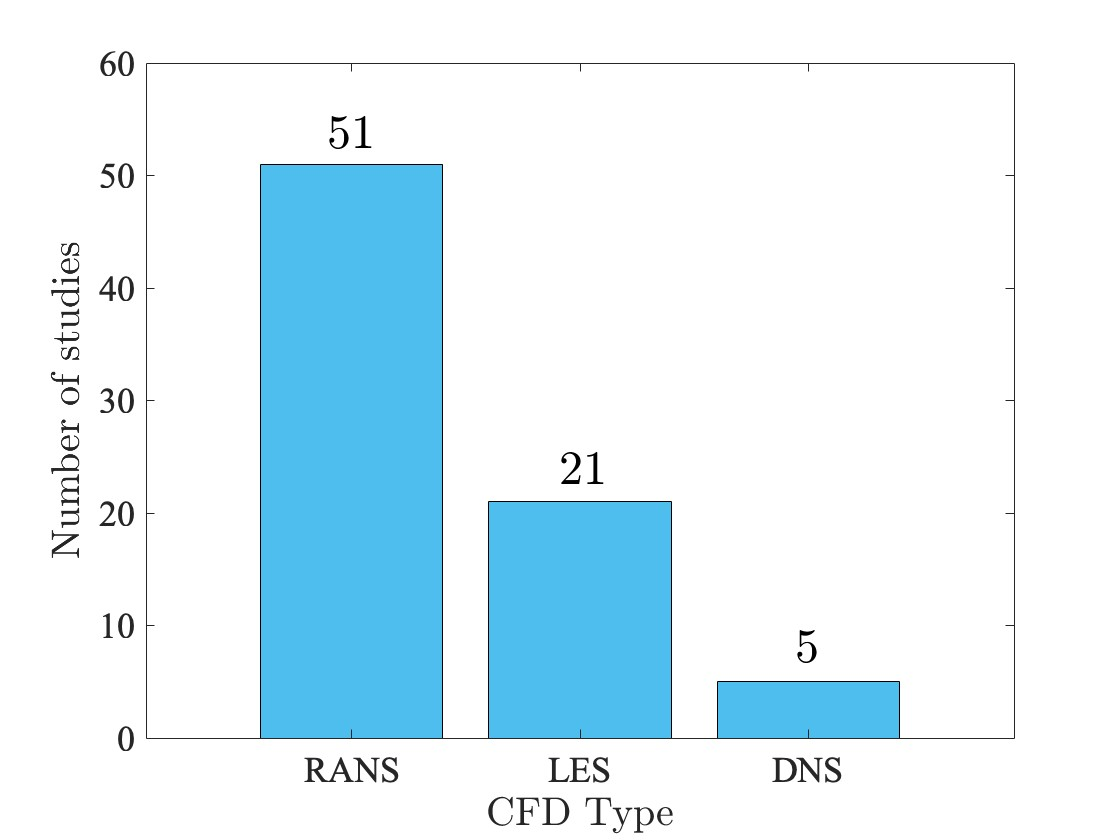
\includegraphics[width=0.8\textwidth]{figures/cfd.jpg}
    \caption{Bar graph depicting the usage of different CFD approaches in indoor airborne transmission studies.}
    \label{fig:cfd}
\end{figure}

\begin{figure}[ht]
    \centering
    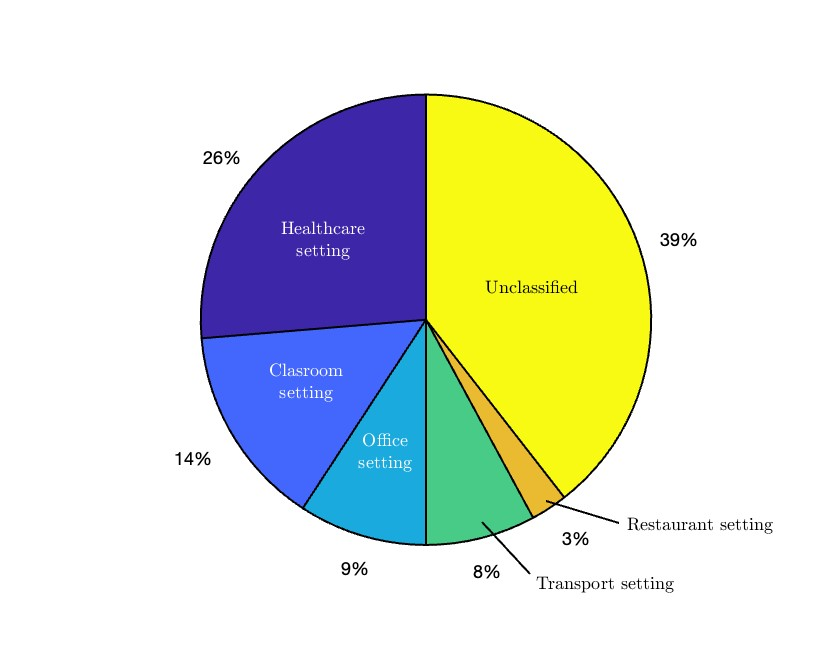
\includegraphics[width=0.8\textwidth]{figures/pie.jpg}
    \caption{Pie chart describing the lack of attention to restaurant settings}
    \label{fig:pie}
\end{figure}

After reviewing the relevant literature, It was discovered that approximately 40\% of the studies I reviewed do not consider a specific indoor setting. The rest of the studies on indoor settings barely consider social settings, especially restaurants. The lack of research for restaurant settings is clearly illustrated in Figure \ref{fig:pie} compared to the various indoor settings. The studies are focused on settings that are adversely affected by pathogen outbreaks that are spread via the airborne route. Still, in the context of a post-pandemic scenario, I prioritise social settings like restaurants for research on indoor airborne transmission. 

Another major shortcoming in research is the effect of occupant dynamics on the flow inside an indoor setting. Most studies studying indoor airborne transmission assume perfectly still occupants, while some studies look into monotonous movements or short sequences of movements. Monotonous movements like walking down an aircraft aisle or inside a patient wardroom, while short movements could be opening a door, walking inside a room and then closing the door. These occupant dynamics are oversimplified, and the time scale of such movement is of $\BigOSI{}{\milli\second}$ which perturbs the indoor airflow for a time scale of $\BigOSI{}{\second}$.

Droplets are the primary carriers of pathogens from an infected occupant to a susceptible one, but their evolution hasn't received enough attention in the past. When an occupant speaks or breathes, they produce droplets of various sizes. These droplets evolve with time from the moment they are emanated due to physical phenomena like evaporation, condensation, and coalescence. Very few studies have looked into this evolution of large droplets to small droplets and vice versa, even if they have discussed the existence of different-sized droplets.

When inhaled by a susceptible occupant, the pathogens carried by the droplets infect them if the quantity of inhaled pathogen exceeds a minimum pathogen load. Calculating the risk of infection involves the probability of inhaling this quantity of pathogen load. From the literature, I found that the risk of infection is often considered the same as exposure to pathogen-laden droplets. Whereas the risk of exposure is the probability of pathogen-laden droplets reaching the breathing zone of the susceptible occupant. They are not the same; thus, quite a few studies have overestimated the risk of infection.

Researchers have tried to quantify airborne transmission in indoor settings for many years and have come very far. However, there is still a lack of qualitative indicators that depict the journey of aerosol from an infected occupant to a susceptible one through a ventilated indoor setting. Visualizing the droplet trajectory is essential in understanding the pathways of the pathogen transmission that can aid in optimising room layout or designing rooms with improved ventilation regimes. It also helps visualise airborne transmission routes in indoor settings to the masses.

The next step for further studies that attempt to quantify airborne transmission is to model the respiratory jet emanating from every occupant in the room. This might block or enhance the transport of infectious aerosol from an infected individual to a susceptible one. The blocking or enhancing effect is even more significant in social settings like restaurants where the occupants are packed closely and engage in increased vocal activity. In these settings, the resultant airflow affects the respiratory aerosol dynamics and, consequently, the extent of long-range airborne transmission, making ventilation strategy optimisation a primary focus for future studies.

Certain weaknesses in the modelling need to be addressed in the future: First, the most energetic and large eddies of indoor turbulence need to be resolved and not modelled. The large eddies represent most of the turbulent kinetic energy spectrum of the flow in a social setting. LES is perfect for capturing these large-scale turbulent structures in the range of Reynolds numbers found in these settings. With more representative flow simulations, incorporating temperature and humidity models to simulate droplet evolution and dynamics is the next step. The effect of occupant movement in long-range transmission is often dealt with in a pre-orchestrated manner. Using AI techniques to enhance CFD reduces the computational costs of complex multiphase flow simulations and handles uncertainty.

Quantifying airborne transmission involves the spatial movement of pathogen-laden droplets, which depends on the airflow in that indoor space. The overlap between ventilation flow, respiratory jets and thermal plumes in Section 3 has been summarised using three of the many occupant configurations and three of the most commonly used ventilation regimes. Table \ref{tab:mat} highlights the potential of mixing between these airflow sources when they interact. The variation among the nine selected settings because of the room's geometry, ventilation regime, occupancy, occupant orientation, and respiratory activities result in unique airflow patterns. These unique airflow patterns can carry infectious aerosol in different room regions, creating hotspots that depend on the aforementioned parameters. Among the scenarios, restaurant settings are the least investigated indoor spaces despite being a hub of social activities with more occupants, more intense respiratory activity, and facing each other.

The dominant airflow patterns carry pathogen-laden aerosols, and as mentioned in Section 4, the droplets evolve while propagating through space. Hot and humid conditions result in a droplet distribution that stays suspended at the head level of the occupants for a long time. Furthermore, humans produce numerous droplets of different sizes when speaking, resulting in the suspension of smaller droplets and ballistic movement of the larger ones. Therefore, human speech in hot and humid conditions has a very high potential to transmit infectious diseases to surrounding occupants via droplets. It explains the widespread airborne transmission of the SARS-CoV-2 virus in tropical and subtropical cities of Brazil \cite{prata2020temperature}. 

There have been numerous attempts by engineers, scientists, and medical doctors to quantify airborne transmission through experiments, CFD simulations, theoretical models, and epidemiological studies. Commercial CFD tools have been used to model indoor airflow and droplet physics for risk assessment or optimization of occupant layout in a room. Experiments, on the other hand, have been used to validate the CFD solver. Certain weaknesses in past modelling techniques fail to capture the flow and droplet physics accurately. For example, Tracer gas experiments fail to account for the non-elastic and volatile behaviour of respiratory droplets, for which I think using pulsatile aerosol generators that can closely mimic the respiratory jet. While RANS simulations average flow turbulence, I suggest using Large Eddy Simulations to resolve the large energetic eddies and model the small ones to be computationally efficient and numerically accurate.

Social settings like restaurants have a high potential for airborne transmission, especially in tropical countries, and conventional ventilation strategies need to be optimised to minimise the spread. The qualitative description of airflow patterns and droplet distribution in various indoor environments is a good starting point for designing an optimal ventilation strategy. Quantitative tools determine the exact development of the turbulent flows and obtain a probability of exposure for the occupants, thus providing data for further fine-tuning. The results from the optimisation help HVAC engineers and planners develop ventilation solutions in social indoor spaces that minimise the time infectious aerosols stay suspended in the air surrounding the occupants. This gives public health organisations precious time to implement active measures to contain an outbreak.

%% The Appendices part is started with the command \appendix;
%% appendix sections are then done as normal sections



%% If you have bibdatabase file and want bibtex to generate the
%% bibitems, please use
%%
 \bibliographystyle{elsarticle-num-names} 
 \bibliography{cas-refs}

\appendix

%% else use the following coding to input the bibitems directly in the
%% TeX file.

% \begin{thebibliography}{00}

% %% \bibitem{label}
% %% Text of bibliographic item

% \bibitem{}

% \end{thebibliography}
\end{document}
\endinput
%%
%% End of file `elsarticle-template-num.tex'.
